\documentclass[11pt,notitlepage,openany,oneside]{book}
\usepackage{ibook}
\includeonly{TEXT/C02/Ch02, TEXT/todo}

\begin{document}

\title{An Idiosyncratic Introduction to Isabelle for Mathematicians}
\author{John Hughes}
\maketitle 
 
%\begin{abstract}
%Starting from Robin Hartshorne's book, we prove things.
%\end{abstract}

\tableofcontents

\chapter*{Origin Story}
This text arose from an attempt at a formalization of Robin Hartshorne's \emph{Foundations of Projective Geometry}
using the Isabelle proof assistant, primarily relying on Isar. That project got started in 2018, continued through a small course in 2020 (interrupted by the pandemic), and restarted in 2023. As a former mathematician, I chose Hartshorne's book because of its relative simplicity -- a projective geometry is a far simpler object than, say, a field or a module, and at least in its simplest form doesn't require any algebraic objects at all -- just four simple axioms about a pair of sets. It seemed as if it should be easy to formalize, especially for someone who happened to already know some ML (the language underlying Isabelle) and who was once a mathematician, hence familiar with proofs. 

It wasn't easy after all, but the problem wasn't either the complexity of projective geometries or my experience with ML and mathematics -- it was a lack of a text that told me enough about Isabelle to let me learn it systematically from the point of view of someone who wanted to do mathematics, but had little interest or experience in formal logic. Many of the texts describe how to prove things about \textit{programs}, which is generally interesting, but tends to use a lot of induction. Hartshorne's book, by contrast, uses induction only once, and it's an induction on a sequence of nested types rather than an induction over some single type or data structure. Many books also take examples from logic, which I found baffling, as I was struggling to understand the difference between Isabelle's 'metalogic' and the 'object logic', and the simple logic theorems used as illustrations were often confusing to me. 

As I've gradually begun to gather a more systematic understand of Isabelle (with a great deal of help, and some other sets of notes like this one), I've begun writing this book, making sure to retain my innocence: a proper degree of confusion about what to do next, something that experienced Isabelle users lack. They say things like ``this is an ordinary co-induction!" or ``prove that `there-exists' proposition by just providing a witness," but they fail to realize how very much is wrapped up in such a telegraphic suggestion. Hence I've written this rather wordy and slow-moving introduction. 

\chapter* {Preface}

I'm assuming you're reading this because you want to try using a proof assistant (PA) and like me, you're someone who already knows how to write proofs of interesting things. My own interests are geometry and topology, just to set some context. I ``learned logic" in 10th grade when we studied Euclidean Geometry. Since those days, I've drifted off and become a computer scientist, and nowadays proof-assistants are used to show many things about computer programs (e.g., ``This program terminates on any input" or ``the state of this filesystem after a `save' operation is what you expect it to be" or ``if you reverse a list twice, you end up with the list you started with."), but those kinds of proofs hold almost no interest for me.

They are (especially the last one) the starting point for most presentations about proof-assistants. The proofs are usually inductive, and many PAs have really great tools for doing inductive proofs. So the introductory presentations harp on and on about induction, and I just can't get much out of them. I've written several papers in math journals, and none of them use induction, and I assume this is true for a lot of mathematicians. 

Other introductory texts on PAs concentrate on \textit{logic}. I know about things like ``modus ponens'' and truth tables and showing that $p \implies q$ is the same as $\neg q \implies \neg p$. But again like many mathematicians, I don't know much about the modern study of logic. I don't lose sleep over the axiom of choice, or constructivism. I mostly just want to get on with proving things about manifolds. But these logic-motivated books tend to start with 30 pages of examples that appear in logic texts, like the theorem that $p \implies  (p \implies p)$ and show how to prove them, and my eyes glaze over once again. 

My goal in writing these notes is to help others like me who want to use a proof assistant, and I'm writing about Isabelle because it seems like the one most likely to be useful to me. 

Of course, some understanding of some logic is necessary to make progress with Isabelle, so I'll have to discuss it at some point. 

I'll introduce what I know of Isabelle through proofs of really silly little theorems, so that the main problems I'm addressing are 

\begin{itemize}
\item Translation from mathematical writing to Isabelle

\item  Learning a useful subset of the syntax and semantics of Isabelle, possibly oversimplified, but enough to get you started down the road. 
\end{itemize}

My experience is that Isabelle is hard to learn, partly because various words are used in ways I find peculiar and hard to remember. I started playing with it six years ago and still find myself asking very basic questions. I feel a bit like Lenny in Steinbeck's \emph{Of Mice and Men,} constantly saying to his brother ``Tell me about the rabbits, George." The only thing I've really learned about learning Isabelle is the importance of learning by doing. 

Much of the Isabelle code here is in the form of images in the document. That's partly so that you get to see the formatting that Isabelle provides, which is great. But it's mostly so that in trying it out, you will actually type it all in for yourself, learning patterns of the language by using them. If you don't want to do that, then this isn't the book for you. If you're willing to trust me on this, read on. Indeed, while I'll move to `copyable text' at some point in the presentation, if at some stage you feel as if you're not `getting it,' consider typing stuff in for yourself. It builds something like muscle memory (you start to remember that \isi{unfolding} is a keyword!) and it makes you think (``Why \isi{unfolding}  rather than \isi{using}? I don't really understand the difference!") and possibly fix some gaps in your knowledge. 

We'll start with a tour of Isabelle with a little description of what's going on, but if you find yourself asking ``How would I possibly know what to type at this point?", the answer is ``You wouldn't!" But I believe that seeing the bigger picture may help you understand how the tool gets used, so we're taking the tour. 

\subsection{What using Isabelle looks like}

The general idea in Isabelle is that at any moment, there's something you want to show is true (a goal), and to do so, you can take several possible approaches: 

\begin{itemize}
    \item 
You can marshal a bunch of related facts and then combine them, as in ``We've shown that if $x$ is positive, then $f(x)$ is larger than $100$; we've shown that in fact $x$ is at least $2$. Thus $f(x)$ is larger than $100.$" 
\item
You can build up one fact after another, each getting closer and closer to the target statement, as in ``Suppose that $\sqrt(2)$ equals a rational number $p/q$, written in lowest terms. Squaring both sides we get $2q^2 = p^2.$ From this we see that $p^2$ is even. By a prior lemma, that in turn tells us that $p$ is even. We can write $p = 2k$ where $k$ is an integer. Then by substitution, we get $2q^2 = (2k)^2$, \ldots", the 'eventual target' in this case being that our supposition must be false. 
\item
You can start with the left-hand-side of some alleged equality and do lots of steps of algebra to eventually convert it to some desired right-hand-side. (Although many mathematicians are quite good at this, it's not actually a place where Isabelle particularly shines.) 
\item 
You can start with some complex entity and repeatedly simplify it until you get what you want. Think of proofs of trig identities, where one constantly ends up factoring out $sin^2(t) + cos^2(t)$  -- where $t$ could be anything --  and then replacing that combination with the number $1,$ yielding a simpler expression, etc., etc.
\end{itemize}
The facts Isabelle has on hand, the various tools developed to manipulate those, and the syntax of Isabelle proofs itself are the tools we (the user and Isabelle) have to work with to address the goals of our work, the usual goal being ``the theorem we're trying to prove happens to be true". 

Isabelle documents used to be written using \term{apply scripts}, which feel like the assembly language of logic. More recently, they're mostly written with Isar, which is a higher-level way to express things. It's still a long distance from natural language, and Isar proofs are sometimes peppered with fragments that look a lot like apply scripts (just as the C programming language once had an ``asm" keyword that introduced fragments of assembly language in the midst of your C code!). But part of my goal in writing these notes is to start with Isar, bringing in the lower-level details only when necessary. 

You'll be forgiven for thinking initially that as a `proof assistant,' Isabelle is a failure -- it seems to be more of a proof \textbf{obstructor} than a proof assistant! You may find yourself in a situation where Isabelle says that some thing is a known fact, and that it's also the goal to be proved. ``Why?", you'll scream, ``Why are you not saying we're done in that case? What more do you want?!?" That's not a situation that helps you advance your mathematical work.  

On the other hand, because of some deep theorem in logic, you can have a lot of confidence that once Isabelle says a proof is correct, it really \textit{is} correct: there's no circular reasoning or logical flaws like proving the converse rather than the contrapositive. So once you become facile with Isabelle, it really does have some value. 

Does it help you do math? My own limited experience says, ``No, not yet." If you're not yet very confident about proving things correctly, or you have really messy things with a ton of cases and want to be sure you didn't miss one, it's probably got some value in 'doing math.' Sometimes writing a theorem in a way that's easy to work with in Isabelle can be an enlightening experience as well, so there's that. 

That brings up another point. There's an old joke about a guy who needs a suit to attend his brother's wedding. The tailor says he'll have the suit ready Friday afternoon, which is good, because the wedding is Friday night. The guy goes to pick up the suit on Friday afternoon and one leg is longer than the other. The tailor says, ``There's no time to fix it, but if you walk with your right foot on tiptoe and your left one flat, it looks fine." Then the guy tries on the jacket, but it's too tight across the back. ``No problem," says the tailor. ``Just throw your arms back and stick out your chest." Then the guy notices that the two sides of the collar are uneven. The tailor tells him to just lean to the right enough that it looks symmetric around his neck. So the guy leaves the tailor shop, arms thrown back and chest pushed out, head tilted over to one side, and hobbling along in a kind of bouncy irregular walk. Two women on the other side of the street notice him, and one says, ``Oh, dear. Look at that poor deformed man. What a hideous life he must lead!" and the other says ``Absolutely, but at least he has a genius for a tailor!" 

Sometimes Isabelle feels that way to me: you take some nice mathematics, and to formalize it you have to twist it almost beyond recognition. At that point, the proofs become easier, but the mathematical ideas are almost unrecognizable. You'll find me mentioning the tailor more than once in these notes.

To be honest, though, a lot of the time using Isabelle feels a bit like a computer game, and you can find yourself up late and night saying ``Wait! I'll just prove \textit{one more} little lemma before I go to bed!" It's pretty addictive, and I think that's a good thing, and it's why I pushed myself to learn more of it.  

\subsubsection{Credit}
Even in its current infantile form, this set of notes make sense in part because of the help I've received from a bunch of folks --- there are whole sections that are nearly verbatim from emails they've sent, or answers they've given on Zulip Chat, etc. First among these is Manuel Eberl, who has been willing to guide me through forests of ignorance. Gunnar Teege's own notes on Isabelle (and email exchanges) have been very valuable. Dan Dougherty and Tim Nelson have both helped me realize how little I know about logic and improved that situation immensely -- Dan seems to have a talent for knowing the language that I'll understand when he's explaining things, and if you look up ``patience" in the dictionary, you'll find Tim's picture. Eugene Stark marked up a few hundred lines of Isabelle that I wrote in about 2018 -- documents so horrible that they must have made his eyes bleed -- and either made notes on or rewrote large sections, helping me learn some of the idioms and approaches that I now rely on. Mathias Fleury's numerous and helpful comments in Zulip chat have also had a substantial influence on the form and content of these notes. 
\chapter{An Isabelle tour, and a first proof or two}

%% sys
%% co
%% figures

\section{Introduction}
Let's take a quick tour of the Isabelle interface, learn a little bit about how to enter text into an Isabelle document, and write a proof of a simple theorem (using tools you won't completely understand because this is a quick tour, not a tutorial). That will give us a chance to see how Isabelle relates to the mathematics you're used to writing. 

This tour will need to introduce things at a bunch of levels -- how do you type that character? What do the colors mean? What kinds of math can I type at \textit{this} point in the file? I'll be answering \textit{some} of the questions at each level, the ones I think are most important for getting started. But you should be prepared to finish the chapter with a lot of unanswered questions.

\subsection{Formatting and style}
The text in this book uses formatting as a guide to content. New terms, for instance, are introduced with \term{this format}. \isi{Isabelle source material} (which I'll also call `code') is in a monospace font with a grey background. Parts of the Isabelle interface like names of \sys{buttons}, menu-options, or panels, have a light-blue/purple background. This is also used for things Isabelle presents as feedback (e.g., the contents of the \sys{Output} panel) except in the rare cases where these are actual Isabelle code. Things related to your computer outside of Isabelle --- directory/folder names, file names like \co{MyTheory.thy}, etc. --- are monospace with a peach background. Because such filenames can also be part of Isabelle code, I won't be completely consistent about this, but I'll try to at least be sensible.

I hope you'll treat reading this book as an \emph{interactive experience}, one where every time you see something new, you'll try it out. To encourage this, I'll sometimes include \term{tasks}, which are things I want you to do right at some particular moment in your reading. The end of a task is marked with a black square. Here's a first one:

\task
As you read this chapter, use Isabelle to do exactly what's described in the text. When I say ``Now delete both \isi{sorry} and the \isi{thm} line,'' you should be editing the text in an Isabelle editor-buffer. Your first step, and the one I am least able to help you with, is to start Isabelle on your computer. 
\etask

Pretty much everything in this book looks the same in Isabelle2023 and Isabelle2024, and will probably look very similar in Isabelle2025. Pick the current latest stable edition of Isabelle, install it, and start it to complete the task. If you're on a Mac, you may have to grant Isabelle various permissions in the Mac's\co{Control Panel...Security} interface to make everything work properly. 

Once you've started up Isabellel, you'll see an interface that looks like this:
\begin{figure}[h]
    \centering
    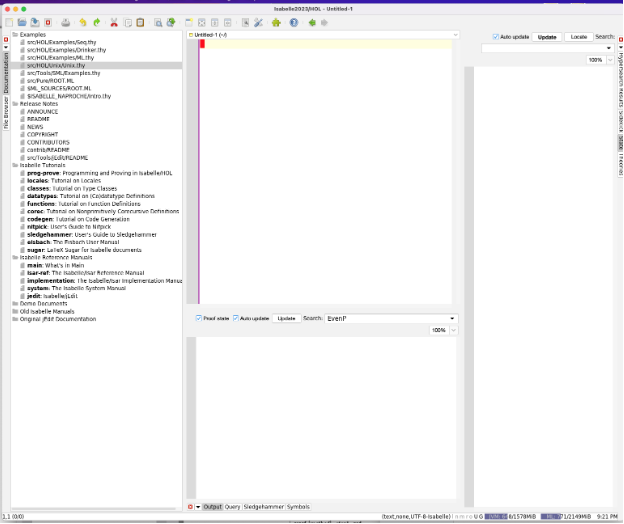
\includegraphics[width=0.7\linewidth]{TEXT//C01//Images/interface.png}
    \caption{The Isabelle interface (as of May 2024)}
    \label{fig:C1-interface}
\end{figure}
In the left column are various documents you can look at. About halfway down, in bold, is \textbf{prog-prove}\textit{\textbf{,}} a book about programming and proving in Isabelle/HOL, which will almost certainly be useful to you at some point, as it is to me. But when I first tried reading it, I rapidly gave up and decided that someone needed to write \textit{this} book instead. 

The top half of the center column is an \sys{Editor} panel -- in it you can type Isabelle documents (which Isabelle folks call \term{theory documents} or \term{proof documents}). As you do so, other threads of execution are constantly processing what you've written and changing the appearance of the editor text -- perhaps color-coding some text, or making red marks along the right-hand side of the document, or generating \textit{output}, which is one of the things that you can see in the other center-column window at the bottom. You can see above that I've got \sys{Output} highlighted; you can actually select \sys{Query}, \sys{Sledgehammer}, or \sys{Symbols} instead. For now, let's stick with \sys{Output}. 

Right here I want to have you do something important. 

\task
Near the top right of the 
\sys{Output} panel, you can see this:
\begin{figure}[h]
    \centering
    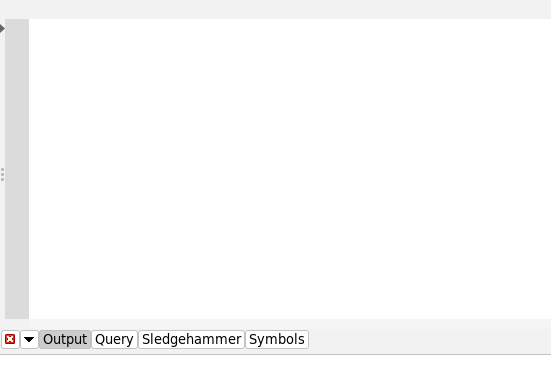
\includegraphics[width=0.75\linewidth]{TEXT/C01//Images/image.png}
\end{figure}
\textit{Be sure that \sys{Proof state} and \sys{Auto update} are both checked.} 
\etask

In everything I write from now on I'll assume that you've done this, so do it now! [Why? Because as you work, you'll constantly be looking at this panel, and having it update as you type, rather than requiring a cursor-motion-and-click, is really nice. Checking \sys{Proof state} says that you'd like to see a little more than the bare minimum feedback, which saves you from looking at \textit{another} panel all the time.]

Moving on, there's the column on the right. \sys{Auto update} is checked, because that's how you'll usually want things. At the right hand side are choices of what to display in the main panel of that column: \sys{Hypersearch Results}, \sys{Sidekick}, \sys{State}, or \sys{Theories}. For now, we'll go with \sys{State}. Down at the bottom are some bits of information: the current time, how much memory various parts of Isabelle are using, etc. 

In the middle column, the top panel shows the currently-active file-name at the top (\co{Untitled-1 (\~/)}; if you look to the right of that filename, you'll see a down-arrow that you can click to discover that there may be other editor buffers available for you to look at as well. When I click on mine, I see this:
\begin{figure}
    \centering
    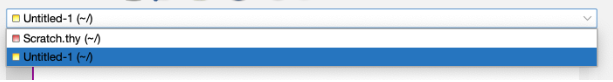
\includegraphics[width=1\linewidth]{TEXT/C01//Images/file-list.png}
\end{figure}
which tells me that in addition to the \co{Untitled-1} document, I've also got open \co{Scratch.thy}. By moving my cursor over that file name and releasing, I can switch to showing that document if I like. Using the \sys{File} menu, you can open a new document (it'll be called \co{Unititled-2}) and toggle between the two of them if you like.

In general, dropdowns like this abound. There's another at the top of the lower center panel, and near the top of the right panel. 

It'd be nice to start writing a theorem and proof, but such things must be contained in a \textit{theory file} for Isabelle to process them. So let's save \co{Untitled-1} (type command-S (Mac) or ctrl-S (Windows)) to do so. You'll see a dialog appear. Mine shows that the file will be saved in \co{/Users/jfh}, but I could navigate around to save it somewhere else. It also shows (at the bottom of the dialog box) that the file will be called \co{Untitled-1}:
\begin{figure}[h]
    \centering
    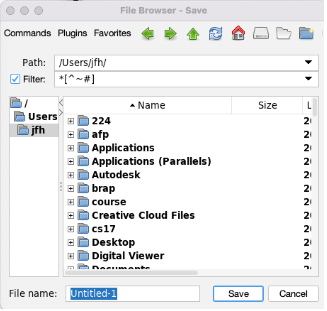
\includegraphics[width=0.5\linewidth]{TEXT/C01//Images/file-chooser.png}
\end{figure}
Let's change that to \co{IBookCh1.thy}, where \co{IBook} means `Isabelle book', \co{Ch1} means `Chapter 1', and \co{.thy} is the extension \textit{required on all theory files}. Without this extension, nothing will work. So let's suck it up and type it in:
\begin{figure}[h]
    \centering
    
\includegraphics[width=0.75\linewidth]{TEXT/C01//Images/file-name-edit.png}
\end{figure}
and click \sys{Save}. 

Two things happen when we save the file: the document title at the top changes to \co{IBookCh1.thy (~/)}, and the cursor in the document becomes bright red:


\begin{figure}[h]
    \centering
    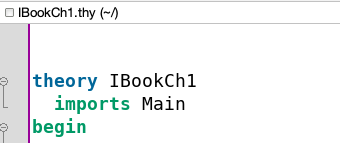
\includegraphics[width=0.5\linewidth]{TEXT/C01//Images/interface-update.png}
\end{figure}
Less obvious is the appearance of a purple line down the left side of the document. 

\digression[File paths]{
The filename above makes sense, but what about the \co{(~/)} after it? In Unix-like operating systems like MacOS, every user has a `home directory' where their files are stored. In my case, that directory is \co{/Users/jfh}. But there's a Unix-standard abbreviation for that, namely a tilde. So \co{\ ~/names.txt} is a way of describing a file called \co{names.txt} that's in my home directory. In the snapshot above, what you're seeing is that there's a file called \co{IBookCh1.thy} in my home directory, the 'directory path' being shown in parentheses at the right. }

\digression[File names]{
The filename may have made sense, but it's not very readable. Why not use some blanks, or hyphens to improve readability? Because those cause problems for Isabelle. Stick with letters, numbers, and underscores in your file names (except for the \co{.thy} at the end, of course).}

We can now start creating our theory document. There are very strict rules for this, rules that I'll enumerate in a little while, but for now, we're just going to type. Here's a start for our theory:

\begin{figure}[h]
    \centering
    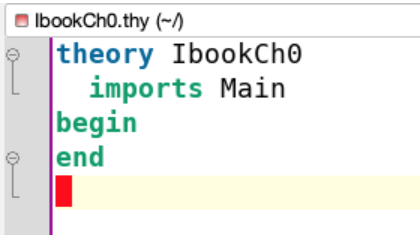
\includegraphics[width=0.5\linewidth]{TEXT/C01//Images/first-theory.png}
    \caption{A first theory document}
    \label{fig:first-theory-doc}
\end{figure}
The theory \textit{must} start with the word \isi{theory}; the theory's name comes next, and it must be exactly the same as the non-extension part of the filename (i.e., the filename except for the \co{thy} at the end). Then comes the keyword \isi{imports}, and then a \isi{begin-end} pair. Isabelle kindly makes keywords be shown in boldface, and does some automatic indentation for us.  As we add more to our theory, the new material will go between the \isi{begin} and the \isi{end}. I've also put a blank line after the end, and my cursor, highlighted in red, is on that line. 

To the left are two small markers that look like a circle with a `$-$' in it, and then a line with a hook. These represent collapsible parts of the document. If I click on the top circle, the display changes to this:
\begin{figure}[h]
    \centering
    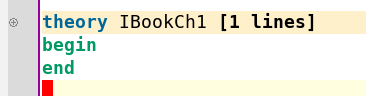
\includegraphics[width=0.5\linewidth]{TEXT/C01//Images/folded-theory.png}
\end{figure}
\noindent which tells you that the first bit of the file has been ``folded up'' and 1 line is now hidden. I can expand it again by clicking on the circled `$+$'. This can be helpful in longer documents for hiding all except the part that you're interested in at some moment. 
\task
Do everything described so far, so that you have your own theory document, and an \isi{imports} line, and a \isi{begin/end} pair,etc.
\etask
By the way, using \isi{imports Main} means that we'll have all sorts of useful facts at our disposal when we want to start writing and proving theorems. An example of this useful stuff is the natural numbers, 0, 1, 2, \ldots  and so on. Those have been defined, and various facts about them proven already, and the theory called \isi{Main} contains these definitions and proofs. (The real and complex numbers are \textit{not} defined in \isi{Main}, by the way; for that you need \isi{Complex_Main}.) You can also leave the space after \isi{imports} blank, but you'll find it's hard to do much of anything, because so many important tools are in \isi{Main}.

Every theory file must have an \isi{imports} line. If you want to import more than one theory, you just write them one after another, separated by spaces. So 
\begin{IS}    
imports Main Complex_Main
\end{IS}
\noindent
is also valid. If you typed
\begin{IS}    
imports Main Tigers
\end{IS}    
\noindent
it'd be a problem, though, because there isn't a theory called \isi{Tigers}. Your interface would look like this:
\begin{figure}[h]
    \centering
    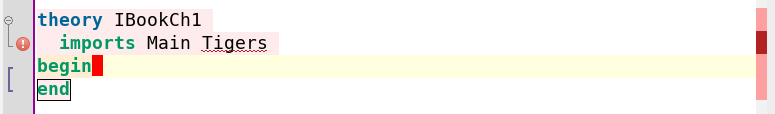
\includegraphics[width=1\linewidth]{TEXT/C01/Images/tigers.png}
\end{figure}
\newpage
And down below, in the Output panel, you'd see this:
\begin{figure}[h]
    \centering
    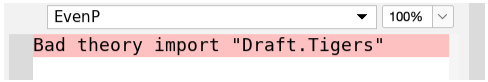
\includegraphics[width=0.75\linewidth]{TEXT/C01/Images/tiger-error.png}
\end{figure}

Or at least you would as long as your cursor was on the \isi{imports} line as shown above. 

What's going on here is that as you're typing, a separate process is interpreting what you've typed, and it's found an error. The red circle with the exclamation point at the left shows the line containing the error. The wiggly red underlining indicates the exact first place the problem occurs. The pink bar to the right with the red rectangle is a schematic picture of your whole document (it's all pink because none of it `works' as a theory file right now), with the location (`near the top') marked with a red bar to tell you where the problem is happening. When your file is 300 lines long, that schematic picture can help you find an error quickly. 

How do you know what theories are available (e.g., \isi{Complex_Main}) and what theories are not (\isi{Tigers})? We'll come back to that. Isabelle has various excellent search tools to help with this kind of question. For now, go ahead and get rid of the Tigers so that our theory file is once again valid. 

\section{A first theorem and proof}
We're now going to state and prove a simple theorem about natural numbers: For any natural number $k$, there's an \textit{even} natural number (i.e., one of the form $2n$) greater than $k$. 

\task I'd like you to pause a moment and think about how you'd prove that. Go ahead and actually write out a proof. (Seriously: do it!) Soon, we'll look at several possible proofs, and chances are good that yours will be among them. 
\etask
To separate that task from my own list of possible proofs, I'll go ahead and talk about how to write this theorem in Isabelle. Between the \isi{begin} and \isi{end} in the theory file, type this: 
\begin{IS}
lemma evens: "\<exists> (n::nat) . 2*n > (k::nat)"
\end{IS}
To do this requires writing a 'there exists' symbol, the inverted E. You do that in Isabelle by typing one of three things:\marginnote{The peach-colored background is there because the isabelle-formatting code used to produce this book converts `\textbackslash\textless exists\textgreater' into the backwards-E, so I had to use a different style.} \isi{EX} or \co{\\<exists>} or \isi{\exists} -- and then pausing until a tooltip offering up the inverted E as a replacement appears. When it does, hitting TAB will complete the replacement. For this particular example, I've included text, and you can simply copy/paste it into the theory file if you choose to do so.

What does the stuff you just typed \textit{mean}? First, \isi{evens} gives a name to your theorem, which you'll be able to reference later. (Isabelle doesn't require a name, but from force of habit, I always name things, and I think it's a good idea.)\marginnote{Often typing some backslash-prepended name will make Isabelle offer \textit{several} replacement options. You can use arrow-keys to move up/down in the list, and then TAB to select one. It appears to me that repeatedly using one replacement will cause it to rise up in the list of choices, at least for a while.} Second, \isi{n::nat} means that \isi{n} is a name for something of type \isi{nat}. This \isi{nat} is the \textit{type} (defined somewhere in \isi{Main}) for the natural numbers. So the first bit is saying ``There's a natural number, $n$, \ldots'', and it's followed by a property of that natural number. The division between the name associated with the `there exists' and the property is the period. So now we can read ``There exists a natural number $n$ \textit{such that} $2n$ is greater than the natural number $k$.'' 

Most mathematicians would prefer to say ``for any natural number $k$, there's a natural number $n$ such that $2n > k$,'' and would find the introduction of $k$ at the end of the lemma-statement a bit weird. 

\subsubsection{Consequences}
Your typing that first theorem caused some changes to appear in the interface. Here's what's going on, taken a piece at a time.

First, the color-coding tells you something. A variable associated with an ``exists'' or ``forall'' is said to be a \term{bound variable}, and they show up in green, as happens with $n$ above. Here's another lemma in which \textit{two} variables are bound by a single ``exists'':
\begin{figure}[h]
    
\includegraphics[width=0.5\linewidth]{TEXT/C01/Images/junk-lemma.png}
\end{figure}

It's a stupid lemma, but it shows the green highlighting. You can go ahead and delete it now. 

In the \isi{evens} lemma, the variable k is \textit{unbound}, so it's shown in blue. And a rule in Isabelle is that any statement like this involving an unbound variable is implicitly universally quantified over that variable, so that this lemma is really saying ``for any natural number $k$ \ldots'' even though that isn't written down anywhere. There's a sneaky detail about the exact nature of that ``for any'', but I'm going to sweep it under the rug for now. 

Again, while you were typing, another process was interpreting and recoloring. Things now look like this:
\begin{figure}[h]
    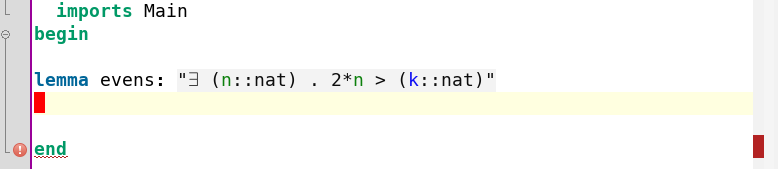
\includegraphics[width=0.75\linewidth]{TEXT/C01/Images/unproved-lemma.png}
\end{figure}
\newpage
(I've trimmed off the top line giving the theory name, and in subsequent images, I'll focus on just the area where we're working.)

The red exclamation and the red bar at the right tell you something is wrong. Even without looking at the \sys{Output} panel below, you can guess what it is: you've asserted this lemma, but haven't provided a proof. In fact the very act of asserting it put Isabelle in a different mode -- one where it wants a proof, and instead it encountered \isi{end}. The output panel tells you this:

There are three things you can do to address this red stuff in the interface, which generally means something is not right:

\begin{itemize}
    \item Write a proof of the lemma
    \item Give up on the lemma by typing \isi{oops} after it, which says to Isabelle ``I don't know how to prove this, so just forget I ever mentioned it, OK?''  That's useful when you're trying to formulate a statement clearly, but haven't yet worked it out in detail, but also don't want to delete what you've written, \textit{or} have it influence anything that follows. If you were writing a computer program, this would be like "commenting out" a section of your program. 
    \item  (somewhat risky) Assert that you'd like to \textit{pretend} you have a proof, so that you can use this lemma in further work, and you'll get back to proving it properly later. For this, you type \isi{sorry}.
\end{itemize}

Obviously the first of these is the best choice, but sometimes we get frustrated and just need to think some more, so the second is a reasonable option: we get to keep the statement of the theorem there in the file so we don't have to remember how to retype those characters, etc., but it doesn't `pollute' anything. The third is the worst: we treat this unproved thing as if it were true, and use it in subsequent work. Maybe we do this because we're sure we can prove it \textit{eventually}, and this lets us make progress. But it's also possible that we've stated it improperly, and as stated, it's actually false! Then we've effectively introduced a new axiom --- that some false statement is true --- into our system, and from that we can prove anything. That's a terrible thing to do to ourselves. Keep that in mind before you use \isi{sorry.} I give this warning because I've done this exact thing! On the other hand, I also use \isi{sorry} sometimes when I should use \isi{oops}. I'm human, after all. 

\textbf{Task}: For now, though, try the experiment. After the lemma, type \isi{sorry}. That word will get highlighted in pink, but you can move on. In fact, you can type \isi{thm evens}, which is a way of asking Isabelle to tell you what it knows about a theorem called \isi{evens}: 
\begin{figure}[h]
    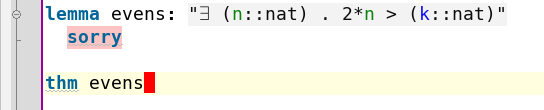
\includegraphics[width=0.75\linewidth]{TEXT/C01//Images/sorry-result.png}
\end{figure}

And down in the \sys{Output} panel you'll get a result:

\begin{figure}[H]
    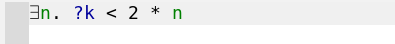
\includegraphics[width=0.5\linewidth]{TEXT/C01//Images/result.png}
\end{figure}

That result looks at least somewhat like our theorem. There's a weird question-mark thing going on, and there's no \isi{\forall k} even though I said Isabelle had one implicitly, and the inequality has been swapped around to use \isi{<} instead of \isi{>}, but it's clearly our theorem there on display. All three of these oddities are things that just happen in Isabelle (for good reasons!), and soon you won't notice them as much as you do at first. 

To finish up, go back and remove both the \isi{thm} line and the \isi{sorry} before it. We've got a lemma stated, and we need to prove it. 

\subsection{Proving our lemma}
Before we do so, here are some possible proofs:

\begin{itemize}
    \item Just pick $n = k + 1$. It's clearly a natural number, and twice it is obviously larger than $k$ (even in the limiting case where $k$ is zero). 
    \item Consider the cases $k = 0$ and $k > 0$. In the first case, $n = 1$ satisfies $2n > k$. In the second, from $k > 0$ we can add $k$ to both sides to get $2k > k$, so $n = k$ satisfies the theorem.
    \item Induction. Again the case $k = 0$ is trivial. Suppose that for some $k > 0$ we have a number $m$ with $2m > k$. We'll show that there's a number $n$ with $2n > k+1$, thus completing the inductive step. Indeed, it's easy: pick $n = m + 1$. Then $2n = 2m + 2  > k + 2$ (by assumption) which is in turn $> k + 1.$ 
\end{itemize}

Your proof was probably one of these, but there are surely others. If yours was different, by all means try to write it in Isabelle, but don't be frustrated if you cannot do so by the end of this chapter: there's an awful lot you don't yet know. 

Let's see one of Isabelle's strong points right here. We're going to ask it to find a proof, and it's going to try a bunch of strategies --- simplification, 'tableau solvers', a reasoner for linear arithmetic, something called a SAT-solver, etc. --- and see what it can come up with. Typing the word \isi{try} makes all this happen. Sadly, especially for new users, \isi{try} sometimes reports that a proof is easy, but doesn't tell you what to type, which is infuriating. Much nicer is \isi{try0}. So right after our lemma, we'll type \isi{try0} (which dispatches a bunch of processes that report back) and wait for a moment:
\begin{figure}[h]
    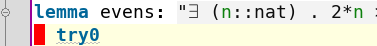
\includegraphics[width=0.5\linewidth]{TEXT/C01//Images/try0.png}
\end{figure}

A moment later, down in the \isi{Output} panel, we see this:
\begin{figure}[H]
    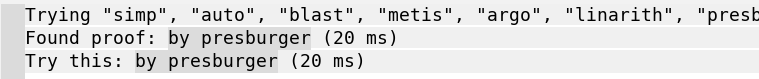
\includegraphics[width=0.75\linewidth]{TEXT/C01//Images/try0-results.png}
\end{figure}

Apparently a proof-method called \isi{presburger} has found a proof. So we can click on the highlighted \isi{by presburger} and it'll be pasted into the buffer. We'll need to backspace out the \isi{try0} to end up with this:
\begin{figure}[h]
    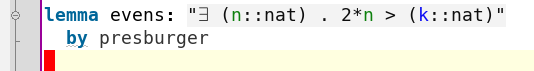
\includegraphics[width=0.5\linewidth]{TEXT/C01/Images/first-proof.png}
\end{figure}
And down in the output window, we have this:
\begin{figure}[h]
    
\includegraphics[width=0.5\linewidth]{output-first-proof.png}
\end{figure}

We've got a theorem (stated a little oddly) and it's been proved. We're done! 

We might, however, be unsatisfied. None of us thought up a proof where we just said \isi{by presburger}, right? Maybe we'd like to use one of the proofs that \textbf{we} came up with, so it can be instructive for future students (not to mention being clear!). We'll do that in a moment, but first let's talk about \isi{try0}.

The nice thing about \isi{try0} is it usually works fast \textit{if} it's going to work at all. And if it \textit{does} work, you can be pretty sure you've stated the theorem right. You may still want to work out a different proof, but at least you've got some confidence. The sad thing about \isi{try0} is that sometimes it seems to be unable to prove the most obvious stuff. To be honest, that's usually because you're using it wrong (e.g., you've asked it to prove something false, perhaps by typing less-than-or-equal when you meant less-than). More on this later. 

There's also that question-mark in front of \isi{k}. How did \textit{that} get there, and what does it mean? Again, we'll look at that later.  For now, here's a brief introduction.

You know that $(x^2 - y^2) = (x-y)(x+y)$, right? Knowing that would let Isabelle, during simplification, transform the left side into the right \ldots \textit{literally}  If Isabelle saw $x^2 - y^2$, it could replace it with $(x-y)(x+y)$. On the other hand, if it say $p^2 - q^2$, it could do nothing. And if it saw $((a+3)^2 - (a+2)^2)$, it could not simplify it to $2a + 5$ using that rule. 
Replacing $x$ and $y$ by \isi{?x} and \isi{?y} says ``this rule can be applied to any pair of \textit{expressions} (of the appropriate type)'', so \isi{?x} could be replaced by $a+3$ and \isi{?y} by $a+2$.

\section{Alternative proofs}
Now let's try to do another proof of this theorem. 

\task Copy-and-paste the lemma, and change the name from \isi{evens} to \isi{evens2}. Move your cursor to the next line and wait a moment, and in the \sys{Output} panel, this appears:

\begin{figure}[h]
    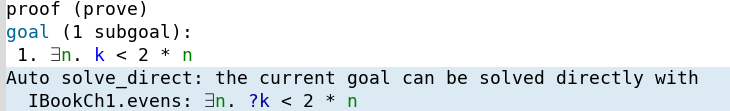
\includegraphics[width=1\linewidth]{TEXT/C01/Images/auto-proof.png}
\end{figure}

Isabelle has done a bit of looking ahead and realized this lemma is particularly easy to prove: it's a consequence of the lemma immediately above (which it has called \isi{IBookCh1.evens}, because we gave it the name \isi{evens}, and it's in a document called \co{IBookCh1.thy}). Unfortunately, it has \textit{not} said how to actually write the proof in Isabelle -- the sort of thing that try0 might have helped with. It turns out that the magic incantation is \isi{using evens by auto} (although \isi{simp} and \isi{blast} could be used instead of \isi{auto} --- any one of them is capable of making the leap from the statement of \isi{evens} to the statement of \isi{evens2}!) Go ahead and type this to see that you've got a second complete-and-proved lemma.
\etask 

\digression[Proof methods]{Isabelle has several built-in proof methods, tools that help us get from what we know to what we want to prove. Names you'll often see are \isi{auto}, \isi{blast}, \isi{simp}, \isi{metis}, \isi{presberger}. Each is good at one thing. The \isi{simp} method, for instance, is good at a particular standardized form of simplification, as the name suggests. For now we're going to aim to use \isi{auto} as often as possible, but when other names pop up in the next chapter, try to just say to yourself ``I suppose he'll explain what that method does at some point.''
}

Let's try to do one of our \textit{own} proofs of the theorem. Once more, copy-paste the theorem statement and change the name, this time to \isi{evens3}. With your cursor after the theorem, the \sys{Output} panel should now be offering you two ways to trivially prove your theorem, but we're going to ignore those. The \sys{State} panel in the right-hand column is showing this:
\begin{figure}[h]
    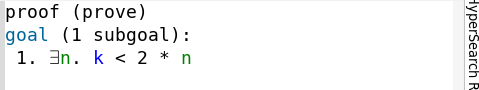
\includegraphics[width=0.75\linewidth]{TEXT/C01/Images/state-panel.png}
\end{figure}

That's telling you a lot. Isabelle has two main modes, `state' and `prove'. (Those are both verbs, not nouns!) In the first, it wants you to state something (which you'll then prove); in the second, it wants you to set about proving one or more things; those things are called \textit{goals} or \textit{subgoals}. In this particular case, we have one goal, which is our current theorem-statement. 

Our prior two proofs are kind of \term{shortcut proofs},  a little bit like when a brief discussion in a textbook concludes with ``we have just shown the following…'', which is followed by some lemma with no further proof. From now on, we're going to mostly avoid those, and our proofs will begin with the word \isi{proof} and end with a matching \isi{qed}. 

To produce the standard kind of proof that we'll generally aim for, we start with the keyword \isi{proof}, followed by something that tells what kind of proof we plan to write (induction, case-analysis, \ldots ). It's also allowable to indicate that we don't have a particular strategy in mind, in which case we write \isi{proof -}.

\textbf{Task}: Add the line \isi{proof -} below your lemma statement and describe how the \sys{Output} and \sys{State} panels have changed. 

We're obliged, at this point, to state something. (Why? Your answer to the previous task should tell you!) We'll generally do so using one of two constructs: \isi{have} and \isi{show}. The \isi{have} construct is for when you want to say something that'll be useful (``$u$ has a unique factorization'') but which isn't one of the current goals. The \isi{show} construct is for when you want to actually establish the truth of some goal (or \term{refine} it -- more on this later). 

Let's commit to one of the proofs, namely the one where we said this:
\begin{quotation}
Just pick $n = k + 1$. It's clearly a natural number, and twice it is obviously larger than $k$ (even in the limiting case where $k$ is zero). 
\end{quotation}
In this case, we're saying that 

\begin{enumerate}
    \item $2(k+1) > k$ (we'll need to prove that), and 
    \item thus there exists a number $n$ with $2n > k$. 
\end{enumerate}
This is a pretty typical situation. We have some proposition (in this case $P(n): 2n > k$), and we want to show that there's some $n$ for which this proposition is true, i.e., we want to show
$$
\exists n . P(n)
$$
We plan to do so by showing that there's a \textit{particular} $n$ for which this is true. (Logicians call this a \term{witness}.) From a logic point of view, we're asserting that
$$
P(b) \implies \exists n . P(n)
$$
And indeed, this is one of Isabelle/HOL's rules for proving things. So let's first establish the truth of the left-hand side here, i.e., exhibit a value of $n$ for which $P(n)$ is true. (We have one in mind, of course -- $k+1$, right?) So we want to say

\begin{IS}
have 2(k+1) > k
\end{IS}
\noindent
i.e., ``we have, as a true-but-yet-to-be-proved fact, that for our natural number $k, 2(k+1) > k.$'' Here \isi{have} is a keyword, and will show up (like \isi{begin} and \isi{end} and \isi{lemma} and other things you've seen) in a bold font in the interface. On the other hand, \isi{"2(k+1) > k"} is not a part of Isabelle's so-called \term{outer syntax}. The general rule is ``stuff like that gets double-quotes'', so we write
\begin{IS}
have "2*(k+1) > k"    
\end{IS}

\task Go ahead and type that on a line by itself and note the change in the Output and in the State panels. Note: the ``star'' for multiplication is essential. Try deleting it and see what kinds of error messages appear; then replace it. Remember this experience though, because sometime in the future you'll again mis-type something in these double-quotes and get a similar error message, which may seem cryptic until you realize that you need to be really careful in writing math for Isabelle.
\etask

When we're marshaling facts like this (it's not really a `fact' yet because we haven't proved it!) it's nice to give them names. We'll see why in a moment. In this case let's give it the name `example', by writing
\begin{IS}
have example: "2*(k+1) > k"    
\end{IS}

\task 
Try replacing the name ``example'' with ``instance''. What goes wrong? 
\etask

We now have a subgoal to prove, and as it's mere algebra without any exponents, 'simp' can probably handle it. We add \isi{by simp} on the next line, and see what happens. The \sys{Output} now looks like this:

\begin{figure}[h]
    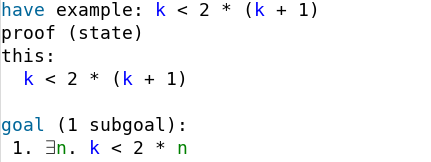
\includegraphics[width=0.5\linewidth]{TEXT/C01/Images/proof-state.png}
\end{figure}

We have a fact called \isi{example}; the current state of things is that we know a fact (the most recent fact is called \isi{this}), and we have a \textit{goal} that we still haven't proved, so we're obliged to do so. With our fact in hand, this \textit{should} be easy. (Note, by the way, that Isabelle has reversed the direction of the inequalities; it always replaces greater-than with less-than!)

This time, we want to assert the overall goal as the next thing to prove, and because we're demonstrating the proof of some \textit{goal}, we use \isi{have} instead of \isi{show}. We \textit{could} retype the overall goal (or copy-paste it from the output panel!) as in 
\begin{figure}[h]
    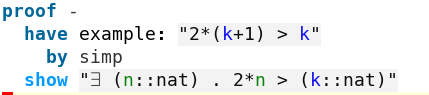
\includegraphics[width=0.5\linewidth]{TEXT/C01/Images/bad-show.png}
\end{figure}

But it's more idiomatic to write this:
\begin{figure}[H]
    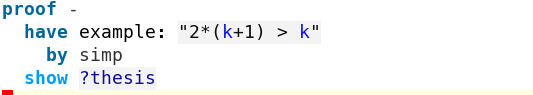
\includegraphics[width=0.75\linewidth]{TEXT/C01/Images/good-show.png}
\end{figure}

That \isi{?thesis} is shorthand for ``the most recent thing we promised to prove'', more or less. 

We can complete the proof with \isi{using example by blast}. The \isi{using} adds the fact we called \isi{example} to the set of things Isabelle can work with, and \isi{blast} does reasoning that includes things like $P(a) \implies \exists x . P(x)$.

A challenge for beginning Isabelle-users is figuring out ``by WHAT???'', because there's \isi{simp}, \isi{auto}, \isi{blast}, \isi{metis}, \ldots  and (a) each of them overlaps with the others to some degree and (b) the names don't really disclose what each one does unless you know more about logic-and-computation than do most mathematicians. I confess that I often use \isi{try0}, so in this case I'd type \isi{using example try0}. The result is a flood of successful proofs:
\begin{figure}[h]
    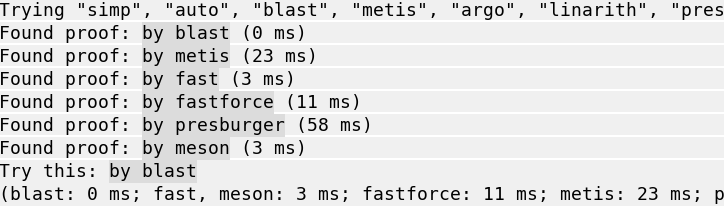
\includegraphics[width=0.75\linewidth]{TEXT/C01/Images/flood.png}
\end{figure}

You can see that this is an easy problem for \isi{blast}, and harder for \isi{fastforce}, and even harder for \isi{presburger} (indeed, that last approach is probably ignoring our 'example' fact and just proving the whole theorem from scratch as it did in the first lemma, \isi{evens}).

And while I \textit{do} use \isi{try0}, I also try to \textit{avoid} using it and get a feel for which solver is the `right' one, as I did when using \isi{simp} to show that $2*(k+1) > k.$ 

So now we have a complete proof:
\begin{figure}[h]
    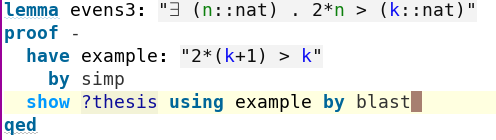
\includegraphics[width=0.75\linewidth]{TEXT/C01/Images/proof1.png}
    \caption{Our first complete proof!}
    \label{fig:first-proof}
\end{figure}

With the cursor in the position shown, the \sys{Output} panel now announces \sys{No subgoals!} and we can add \isi{qed}, which is like a closing-parenthesis for \isi{proof}. If you move your cursor up and down through the proof, you can see how the output changes after each line. 

You will soon grow to love seeing \sys{No subgoals!} It's like being able to check an item off your list of things you need to do -- it feels good! And just as some people enjoy that so much that they begin adding tiny tasks (`Find shovel') to the list before larger ones (`Shovel snow off driveway'), you may find yourself so eager to see \sys{No subgoals!} that you begin proving small things on the way to larger ones. Fortunately, this is an \textit{excellent} strategy in Isabelle. 

Returning to the lemma we're working on, if you change the method used to show \isi{?thesis}, something a bit surprising happens. Change \isi{blast} to \isi{auto} (which cannot in fact do the proof) and you'll once again see that there are no goals left. But something critically important has happened -- red error bars appear on the right-hand side, indicating that this is a place where problems remain. Furthermore, down in the \sys{Output} panel there's an error message telling you that no proof was found. 

What's going on here is that there are multiple threads of execution interacting with this UI, and at least one of them is saying, ``Well, if you say that you've shown something, I guess I'll trust you'' and says that there are no further goals. Another thread might be off looking for a proof of that claim, and simply not have finished the job. (In our case it \textit{has} finished and failed to find a proof, but the idea's the same.) This somewhat peculiar behavior can be both a benefit and a curse. You should get accustomed to looking at those red or pink bars on the right to be sure things have gone as well as you might think that they have. 

Speaking of that, when you load a big theory file -- hundreds of lines perhaps -- you'll see a pink bar at the right indicating that Isabelle has not checked the theory for correctness. Soon the top of that bar will turn white --- Isabelle has checked the part that's visible in the editor panel. As you move your cursor down in the editor, more and more will turn white unless you encounter an error or a place where the proving takes a while to complete. 

\subsubsection{Two more proofs}

We have two more proofs of our lemma still waiting in the wings. Here they are, encoded in Isabelle, for you to look at. I'm not going to explain them in the same detail as the first proof, but you should type them in and step through them, watching how the proof-state changes with each line, as a way of getting a feel for two other proof strategies. 

By the way, none of the proofs in this chapter should be considered models of compactness or excellent style. They're straightforward and somewhat wordy and show some basic Isabelle tools using only a few keywords, and that's intentional. I want to set you up to be able to construct a few more proofs of simple statements on your own. They also follow some conventions like 

\begin{itemize}
    \item Using names for facts, particularly long names
    \item Annotating with \isi{(* \ldots  *)} comments to explain what's going on; usually Isabelle proofs aim for brevity rather than readability.
\end{itemize}

To continue with our small theorem, we have two more proofs: 

\begin{quotation}
Consider the cases $k = 0$ and $k > 0$. In the first case, $n = 1$ satisfies $2n > k$. In the second, from $k > 0$ we can add $k$ to both sides to get $2k > k$, so $n = k$ satisfies the theorem.
\end{quotation}

Here's that proof, in Isabelle:
\begin{figure}[h]
    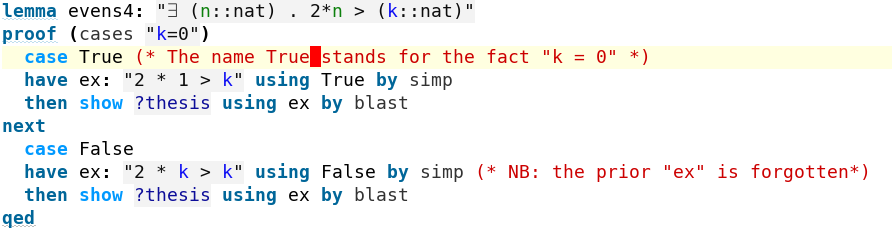
\includegraphics[width=1\linewidth]{TEXT/C01/Images/proof2.png}
    \caption{A proof by cases}
\end{figure}

\begin{quotation}    
Induction. Again the case $k = 0$ is trivial. Suppose that for some $k > 0$ we have a number $m$ with $2m > k$. We'll show that there's a number $n$ with $2n > k+1$, thus completing the inductive step. Indeed, it's easy: pick $n = m + 1$. Then $2n = 2m + 2  > k + 2$ (by assumption). This is in turn $> k + 1.$ 
\end{quotation}

The proof, in Isabelle:

\begin{figure}[H]
    \centering
    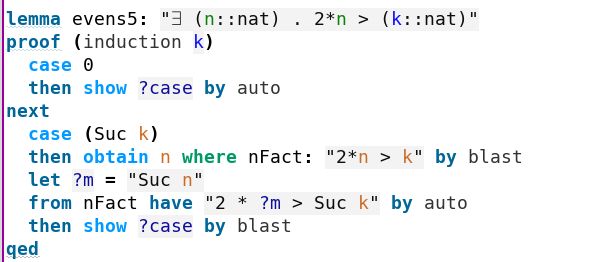
\includegraphics[width=0.75\linewidth]{TEXT/C01/Images/proof3.png}
    \caption{A proof by induction}
\end{figure}

If that last proof looks only superficially like induction to you, you're in good company. You can certainly see that things fall into a base case and an inductive case, and the ``assume $P(k)$'' part of things is somehow all automatically laid out by saying \isi{case (Suc k)}. The rest probably feels just a bit weird, and that's OK. For instance, we no longer have \isi{show ?thesis} but instead \isi{show ?case}. 

Induction in Isabelle is very general and very powerful, but is therefore also a little challenging to use in simple cases, and pretty inscrutable to the beginner.

We've also used \isi{obtain} here. Remember how I said that there's a rule $P(b) \implies \exists x . P(x)$, so that writing down one example for which $P$ is true suffices to show the ``there-exists'' claim? The word \isi{obtain} is the counterpoint to that: it says  that if you know there's an $x$ with $P(x)$ being true, then you can create a name for such an $x$ and use it in the rest of your proof. As an example, the intermediate value theorem says that if $f$ is a continuous function from the reals to the reals and $f(0) > 0$ and $f(1) < 0$, then $f(x) = 0$ for some $x$ between $0$ and $1$. If we'd proved this theorem in Isabelle, we could write \isi{obtain c where f(c) = 0} and use \isi{c} in the remainder of some proof.  

\section{Review}
Let's review a few key points from this chapter:

\begin{itemize}
    \item The UI has three panels -- the editor, the proof-state, and the output -- that you'll use a lot while creating theory files

\begin{itemize}
        \item Color-coding and automatic formatting of text tell you a \textit{lot} about what's going on
        \item There are multiple processes acting on the UI at any moment, and their interaction can occasionally be surprising. 
        \item \textit{\textit{Always} pay attention to anything that's red!}
\end{itemize}

    \item Theory-files have a fixed structure; the name of the theory must match the name of the file; the name of the file must end in \isi{.thy}, and the theory name should contain only letters, digits, and underscores. 
    \item Isabelle uses a lot of special symbols. You've learned how to type one of them using the ``type something, pause, and then hit TAB'' approach, but you'll need to learn more. 
    \item Theory-files have a block structure: each \isi{proof} must be matched by a \isi{qed}; each \isi{begin} must be matched by an \isi{end}
    \item If you can't prove something, \isi{oops} is a good way to tell Isabelle to forget all about it. \isi{sorry} is a less-good way, but frequently useful.
    \item Non-keyword text in an Isabelle document generally needs double quotation marks around it. (We'll learn later to use `cartouches' as an alternative.)
    \item You've seen two forms of proof, one of which omits the word \isi{proof} and simply says something like \isi{by auto}; the other one starts with \isi{proof} and ends with \isi{qed}
    \item Within proofs, there are various 'proof methods' named simp, auto, blast, metis, etc., that are good at different things, and you'll need to learn which ones are good at which things. For now, that's just a big pile of words. 
    \item When you're in a state of affairs that requires a proof (the proof-state panel says \sys{proof (prove)}), you can type \isi{try} or (better in general) \isi{try0} to see whether Isabelle can find an easy proof for you. 
    \item Proofs can have various structures (cases, contradiction, induction, \ldots ) and each has its own way of being written in Isabelle. 
    \item During a proof, there are goals and subgoals, and your aim is to eliminate all of them. 
    \item You've learned about quite a few Isabelle keywords -- \isi{theory}, \isi{imports}, \isi{begin}, \isi{end}, \isi{lemma}, \isi{using}, \isi{by}, \isi{proof}, \isi{have}, \isi{show}, \isi{case}, \isi{let}, \isi{obtain} -- although the details of most are still to be disclosed. 
    \item You're ready to do some proofs on your own as homework or better, as ``drill'' to help get some patterns into your head. 
\end{itemize}

Finally, I want to note that absolutely nothing we've done so far matches a typical use of Isabelle by an expert -- an expert would have started out any project by searching through Isabelle's known theorems (using its powerful search tools!) to see whether the thing they're trying to prove is already known, or at least something \textit{similar} is known and can be used as a starting point. We'll get to this kind of proving later. 

\section{Homework Exercises}

\begin{enumerate}
    \item Create a new theory file to hold a theory called HW1. What should the name of the file be? Make sure to follow the naming rules.
    \item Type enough into the file to make it a valid theory file (i.e., something beginning with the word \isi{theory} and ending with \isi{end}, and having all keywords highlighted by Isabelle.)
    \item Here's a tiny theorem: \textit{For any natural number n, there's an odd number larger than n. }And here's a proof:\textit{ The number 2n + 1 is an odd number larger than n. }

State and prove this theorem using this proof, in Isabelle, using a proof that starts with the word \isi{proof} rather than just \isi{by}. Try to do it without using \isi{try} or \isi{try0}. Call your theorem \isi{odds}. 

\item Change the first word of your theorem statement from \isi{theorem} to \isi{lemma} or vice versa to see that the results are identical. The word \isi{proposition} can also be used. 
 
\item Here's another theorem: The square of any natural number is nonnegative. State and prove this in Isabelle. To write the square of a number b, for now just use \isi{b * b}. Hint: to get the ``greater-than-or-equal'' symbol, type `\textbackslash{}ge' and pause until a completion/substitution is offered, and then press TAB. And to indicate that $n$ is a natural number, use \isi{n::nat}, which must be in parentheses to make parsing reasonable. Go ahead and use a \isi{by} proof, because you don't yet know how to find a theorem that says that the product of non-negatives is non-negative, or that naturals are closed under multiplication, but both are true and known within \isi{Main}. Looking at the hints provided by \sys{Auto solve\_direct} will give you some feel for the kinds of facts that are available to you. 

\end{enumerate}
State and prove the theorem (using this proof) in Isabelle. (By the way, this theorem can \textit{also }be proved using \isi{by auto}, although Auto solve\_direct doesn't find that proof.)

\section{Lagniappe}

Just as the red circle with an exclamation in the left edge of a theory document signals an error, a blue circle with an ``i'' in it tells you that Isabelle has something you might want to know, like the fact that \isi{evens2} was easily proved using the \isi{evens} lemma. 

 

\chapter{More mechanical details and how-tos, and a bit more syntax.}
After the brief introduction of the last chapter, you probably have a bunch of questions, things like 
The math-y stuff in double quotes --- what am I allowed to write in there? Can I use things like "using" and "show"? 
When do I need double-quotes? 
This whole "using" thing seems annoying. Why doesn't Isabelle just keep track of the things I've proved and assume that I want to use those whenever possible? 
We used the name "example" (and later the shorter "ex") for the various facts we accumulated, but what are the rules for those? From trying out 'instance' I could see that using an Isabelle keyword was bad, but is everything else OK? 
How do I type the characters that I need? I can't just wait for you to tell me all of them!
You had me use "Output" and "State" in two of the panels, but what are those other things? 
Do I have to put everything in one theory file?
In all those proofs, you built up stuff to prove the main "thesis", but what about proofs where we work backwards from the thesis, like saying "to prove that for positive numbers n,  2n + 1 > n + 1", it suffices to prove  that 2n > n"? Can we do those in Isabelle? 
Building up proofs in individual steps seems OK, but if a theory file gets big, how will I remember the names of all the things that I can use in trying to write a proof -- is it \isi{plus_commute} or \isi{add_commute}? Can Isabelle help with some of this?

We'll answer some of those in this chapter, and partially answer others. In making this list, I wanted to reassure you that if you feel confused about something, it's perfectly reasonable: Isabelle has a lot of parts, and it's impossible to introduce them all at once, so there'll be pending questions for a while.

Disclaimer
By the way, Isabelle is a system in which something called Higher Order Logic (HOL) is implemented, resulting in Isabelle/HOL, which is what I've been calling "Isabelle". There are other logics implemented in Isabelle as well, such as First Order Logic, and Zermelo-Frankel Set Theory; these result in Isabelle/FOL and Isabelle/Zf, about which I will say no more because I know nothing about them. Furthermore, the interface we'll use is called Isabelle/jEdit, and it's a complex program in itself. But I'm going to be sloppy and use the word Isabelle for this editor, for the Isabelle/HOL language, and for the whole ecosystem. 

You can write a program that links to Isabelle, or even write code within an Isabelle theory document, or ask Isabelle to produce code that implements something that you've proved (in Isabelle) to be correct. I know nothing more about these topics than that they exist, so you won't learn about them in this book. 

Warmup: more mechanics
Looking at the bottom of the center column of the interface, we see this:



with "Output" highlighted because we've been using this panel to see what's going on. 

Symbols
But the "Symbols" tab is also useful. Click on it, and you'll see a selection of choices:

where I've clicked on the choice "Arrow", which shows all the kinds of arrows available in Isabelle. If you move your cursor over one and let it rest there for a moment, a tooltip appears:


and this shows you that to produce that character in your theory file, you may type \isi{\\<Longrightarrow>} (although \isi{\\Longrightarrow} also works), or type ".>" (which doesn't work on my system), or type "==>", which does work. This lets you rapidly assemble a collection of shortcuts for symbols that you use often, and lets you look up others. If you use LaTeX, many of the symbol-names closely match the ones in LaTeX. The most useful of the options in this particular section is probably the one called "Search". Confession: I used this panel to find some favorite symbols, and now seldom look at it at all. 

In practice, I use only a few of the symbols, and below I show my go-to list. You've already seen greater-than-or-equal, and can guess at similar things, I'm hoping. And Greek letters are just given by their names with backslash in front, like \beta.

  [|    ⟦
  |]    ⟧

  \real ℝ
  \int  ℤ
  \nat  ℕ

  ==>  ⟹  
  <>   ⟺

  EX    ∃
  ALL   ∀
  /\    ∧
  \/    ∨
  \not  ¬

  \union ∪
  \inter ∩
  \emptyset ∅
  \subset ⊂

Query
The query tab gives you the ability to find already-proved theorems to use, saving you a ton of work. The only tricky thing about it is the need to press the "Apply" button. So many other things in Isabelle's interface happen 'as you type' that it's easy to forget. Within the Query panel are several choices:


and the one that is probably most interesting to the beginner is "Print Context". If we take a simple theory like this one:

with the cursor position shown in red, and check all four boxes (contest, cases, terms, theorems) and press "Apply", we see this

which helps disclose a little bit of what's going on during processing of a theory document. You can see that the name "?this" has been bound to "n + 1 <= 2 * n + 1", and "?thesis" is bound to the same thing, and that there are some other 'facts' available for reasoning about goals. Try moving the cursor up and down through a proof and clicking "Apply" repeatedly to see a bit more. 

More useful in general is the "Find Theorems" tab in this panel; we'll return to that presently. 

Sledgehammer
Sledgehammer is a proof-finding tool that applies a bunch of approaches all at once, spawning multiple processes; the chosen approaches are named in a list in the Sledgehammer tab. You can place your cursor somewhere in a theory where you need a proof (e.g., right after a theorem statement), and click the "Apply" button in the Sledgehammer panel, and see the results. If in the example above I place my cursor right at the end of the lemma statement and use Sledgehammer, I'll see this produced over the course of a few seconds on my very slow old Macbook:


As you can see, Sledgehammer is a lot like the "try0" that we've been using. But "try0" does a lot less, so it operates faster, but with less power.  Sledgehammer is also, in my experience, one of the parts of Isabelle that's most likely to have failures of one sort or another, but you're unlikely to encounter these during early proving sessions. When you click "Apply" in the sledgehammer panel, you're spawning a lot of computation…which continues until all the various solvers report back that they're done. This can slow things down a lot, so it's a good idea to click "cancel" as soon as you get tired of waiting or get a proof that you feel you can use. Sledgehammer will also sometimes report that one of its provers has found a proof…but then take forever to report what that proof actually is, or perhaps never do so. I'm just warning you that it can be frustrating! 
Sessions
A single theory document is a place to put closely-related items, although the notion of 'closely-related' is of course ambiguous. Does everything about Group Theory go in one theory document? Or do we make a document for finite groups? Or perhaps a single document just for groups represented by generators and relations? That's all a matter of taste. But just as a book gets divided into chapters, there comes a time in the development of some mathematics when it begins to feel unwieldy. In Isabelle, this often happens at the time when loading your theory document starts to take a long time, during which all the initial work is checked even though you're planning to work only at the end. Wouldn't it be nice if you could take the completed part of your theory and store it away, and work on a new part that references that other portion? That's what 'sessions' are for. They serve much the same organizational function that directories/folders serve in a file-system: gather related items together in a hierarchical arrangement. There's a side-effect, though, one that's kind of nice: building a session also sets you up to be able to make a nice typeset version of your theory document. 

Fair warning: this discussion is something you'll read once, then apply by copying a few commands to set up a session, and then forget until the next time you need to do it. With that in mind, let's get to it!

All the files in a session are typically stored in a single directory, which contains all the related theory files and a special file called ROOT that describes the session. Every session has a 'parent' (again like directories in a filesystem), except for the 'starting' session for Isabelle, called "Pure" (the equivalent of the directory "/" on a Linux/Unix filesystem). The ROOT file records the parent session. I'm only going to discuss the default structure for a session; fancier stuff is available in the documentation, but I've never needed it. 

Let's go ahead and create a session. I'll do this on my Macbook; you'll need to adapt things to your operating system. Things after "//" are comments on what's going on; don't type them. All operations take place in a Terminal window. 

A digression on paths: on most systems, there's a notion of a search-path where the OS looks for programs to run. On linux-like systems, that typically involves things like "/bin". On my Macbook, it looks like this:

jfh@jfhs-MacBook-Pro book % echo $PATH
/Users/jfh/.npm-global/bin:/Library/Frameworks/Python.framework/Versions/3.11/bin:/usr/local/bin:/usr/bin:/bin:/usr/sbin:/sbin:/Library/TeX/texbin:/opt/X11/bin:/Library/Apple/usr/bin:/Users/jfh/.rvm/bin

You can see that it's a list of colon-separated paths to various folders where executable programs are stored. If you type

% run-it foo

The OS will search for a program called "run-it" in all those places, and when it finds one, it will indeed run that program with "foo" as a command-line argument. If it doesn't find that name anywhere, it'll say something like "run-it: not found". Isabelle itself has several runnable programs; on a Mac, they're found in "/Applications/Isabelle2023/bin"; one of them is called "isabelle".You can add "/Applications/Isabelle2023/bin" to your path so that this program can be found, or you can change to the directory called "/Applications/Isabelle2023/bin" and type 

% ./isabelle

to run it, or you can type the full name of the program, i.e., 

% /Applications/Isabelle2023/bin/isabelle

All three work. I'll use the last of these. End of digression.

              // create a session on the desktop; be sure 
        //that ~/Desktop/book doesn't already exist!
% /Applications/Isabelle2023.app/bin/isabelle mkroot ~/Desktop/book  

Initializing session "book" in "/Users/jfh/Desktop/book"
  creating "/Users/jfh/Desktop/book/ROOT"
  creating "/Users/jfh/Desktop/book/document/root.tex"
Now use the following command line to build the session:
  isabelle build -D /Users/jfh/Desktop/book

At this point the "book" directory contains a text-file, ROOT, and a subdirectory, "document" with a LaTeX document root.tex in it. 

        // Follow the instruction on the last line to "build the session"
% /Applications/Isabelle2023.app/bin/isabelle build -D /Users/jfh/Desktop/book
Running book ...
Preparing book/document ...
Finished book/document (0:00:28 elapsed time)
Document at "/Users/jfh/Desktop/book/output/document.pdf"
Finished book (0:00:02 elapsed time)
0:00:44 elapsed time

As you can see, that last step is a little slow. So what happened? A bunch of stuff. If we go to the newly-created session, we see this:

jfh@jfhs-MacBook-Pro bin % cd ~/Desktop/book
jfh@jfhs-MacBook-Pro book % ls
ROOT		document	output


Running the "build" created a new "output" directory, and the entire directory structure is now this:

jfh@jfhs-MacBook-Pro book % ls -R  
ROOT		document	output

./document:
root.tex

./output:
document	document.pdf

./output/document:
comment.sty			isabelletags.sty		root.tex
isabelle.sty		pdfsetup.sty		session.tex
isabellesym.sty		railsetup.sty		session_graph.pdf

The contents of the ROOT file are this:

jfh@jfhs-MacBook-Pro book % more ROOT 
session book = HOL +
  options [document = pdf, document_output = "output"]
(*theories [document = false]
    A
    B
  theories
    C
    D*)
  document_files
    "root.tex"

What that's saying is that this session's parent is "HOL", for which Isabelle already has a precompiled 'heap file', which is its way of storing the results of processing all the theory files so that it can load them almost instantly rather than working through each one of hundreds of individual files. Processing a session also creates a heap file -- i.e., it creates a record of everything that results from processing the theory files in that session so that they don't all need to be re-loaded and processed. The ROOT file also says that in creating a pretty document for this session, I want the result to be a pdf, and that this pdf should be put in the folder "book/output". It then, in a comment-block, shows how we might say which theory files are included in this session. In this case, it's indicating that theories A and B should not appear in the output document, but C and D should. And finally, it says that the files used to produce the output document (aside from the theory files themselves) are … well, there's only one, called "root.tex". If you wanted to include a bibliography, you might include "root.bib", for instance. 

If we navigate to the "output" folder and look at the resulting "document.pdf", it's pretty boring:


but that's because there are no theory files in the session. Let's do one more thing, and include our chapter-zero theory file. Let's move that file from wherever you put it to the "book" folder and then again run the "build" process. In my case, the chapter-zero file was in my home directory:

jfh@jfhs-MacBook-Pro book % mv ~/IbookCh0.thy .
jfh@jfhs-MacBook-Pro book % /Applications/Isabelle2023.app/bin/isabelle build -D ~/Desktop/book   
0:00:11 elapsed time

The result is … no change at all in the document.pdf file! That's because we didn't edit the ROOT file to tell it that our session had a new theory. We have to edit that file (use your favorite text-editing tool) to make it look like this:

session book = HOL +
  options [document = pdf, document_output = "output"]
  theories IbookCh0
  document_files
    "root.tex"

Notice that in listing the theories, I have to not include ".thy" in the name! 
Then we can re-run the "build" command and get a document.pdf that starts like this:




Warning: If your theory file contains an error, it's possible that your "build" will fail, and then you need to fix things. If your document contains clever LaTeX tricks, debugging the build process can become a serious challenge, alas. I have no suggestions except that in trade for the beauty of the output, you have to eventually get comfortable with the challenges of the complicated LaTeX typesetting system.

That was a lot of mechanics, but we've mostly addressed items 5, 6, and 7 from the pending-questions list. Let's move on to some more questions about actually proving things. 
More proving: a different style
Isabelle (and in particular Isar) provides another way of stating theorems, one that has a lot of appeal because of its consistency. For our little 'evens' theorem, it looks like this:

lemma evens5:
  fixes k::nat
  shows "∃ n . 2*n > k"
proof -
  show ?thesis by presburger
qed

I've used the simple presburger proof here so that I can concentrate on the statement. For more complicated theorems, there can also be an "assumes" between "fixes" and "shows". But in this simple case, the name k, which was previously universally quantified without our saying anything about it, is made explicit up front. This is meant to remind you of the way you might start when you want to show that "for any k, there's an even number bigger than k." You start by saying "Let's fix some arbitrary natural number k, and then …" 

Digression on getting theorem statements right
Let's suppose you want to show that for positive n, we have 2n + 1 > n + 1, and you write

lemma "dominate": " 2* (n::nat) + 1 > n + 1"
  by presburger

filling in the "by presburger" based on your experience with showing this sort of thing. 
Go ahead and type this in, and see what happens. 

You'll notice two things: the proof has a red circle to its left, with  'presburger' underlined with a red squiggle, and the theorem itself has a blue "i" next to it. If you place your cursor on the lemma statement, you'll see in the output window 

That's telling you that a background process has been checking the theorems you're claiming, just to see whether it can find an easy counterexample. In this case, it came up with n = 0, which is indeed a natural number for which the alleged theorem's not true. This can be a big help in getting theorem statements right. <End of digression>

We can restate that "dominate" lemma in fix-assume-show form:

My experience is that this structure helps me remember to assign types to things (in the "fixes" line), and to write down all hypotheses (in the "assumes" line). I've omitted writing a proof because I want to use this example later to show a different style of proving from the ones we've seen so far. 

There's a corresponding proof structure to the theorem-stating fixes-assumes-shows pattern. It uses the imperative form of the three verbs: fix, assume, show. We'll return to this in Chapter XXX.

Each of the three parts of a fixes-assumes-shows theorem-statement can also contain "and", or can be repeated, so "fixes n and k" is acceptable, but so is 
  fixes n 
  fixes k
Here's a very silly example making two claims about some natural numbers, showing how "and" is used. 



Two notes are due here.
Generally showing two or more things isn't a great idea. When you later refer to the theorem, Isabelle has to guess which conclusion you think is relevant in the current situation. Of course, if there's some complicated set of hypotheses that you don't want to repeat multiple times, and that leads to several facts (e.g., a theorem of the form "If we know A, B, and C, then the following 5 statements are all equivalent"), it's OK to write such a theorem. But don't do it unless you need to. (To be fair, I'll be violating this first suggestion in a page or two!)
If in my silly lemma I had replaced the second conclusion with "n * k > 15", I'd have been stuck -- nothing we've learned about yet shows how to prove such an inequality. I'm deliberately concentrating for now on the structures of proofs rather than the use of existing theorems to prove new ones. 

Practice
You're now going to practice writing theorems using the fix/assume/show format, and then proving them using the few tools you've learned so far. To supply a meaningful example, I've taken part of the first chapter of Michael Spivak's Calculus, which introduces an axiomatic formulation of the real numbers, and encoded it in Isabelle. (The book, at least in early editions, is widely available as a PDF download.) Spivak shows how to use the axioms to prove some small results, and I've imitated some of those proofs (almost verbatim) in Isabelle.

Open up the IbookCh1_starter.thy file and take a look at the first few lines, and then continue reading here.

One challenge here is that the natural numbers and integers, and their associated notions of addition and multiplication are already present in Main, and I want to be sure that Spivak's discussion isn't polluted by those. To do so, I've declared a new type, named "r" (for "real"), to serve as a proxy for the real numbers. When we declare a new type, we're guaranteed two things: there is at least one value of that type, and any value of our new type is different from any value of any previously-existing type. So it gives us a clean slate to work from. 

Initially we know virtually nothing about the type r, but I've used the "sorry" feature of Isabelle to allow me to make statements about elements of r that will be taken as true henceforth. (Yes, I warned earlier about the perils of "sorry" and how one might accidentally introduce inconsistent 'truths' by using them. But I'm pretty confident that the axioms of the reals are not, in fact, contradictory, so I'm happy to do this for this example.) By the way statements to be taken as true henceforth are called facts. 

There's an alternative Isabelle construct -- axiomatization -- that I could have used for the same purpose, but it's generally reserved for quite specific tasks like defining a new logic, and I don't expect to ever use it in my Isabelle documents, so I wanted to avoid using it here. Let's see how things start out:

I've said here that there's a new type called "r", and that there are six "constants". The first four are functions called plus, minus, neg, and reciprocal; the last two are single elements of r to which I've given the name Z (suggesting 'zero') and U (suggesting 'unit', and which is supposed to act as 'one'  in our number system, but abbreviating with the first letter and getting "O" seemed like a really bad choice for something that was representing "1"). A constant is simply a name that will be used throughout a document to mean a single thing. Their use is relatively rare in Isabelle, but appropriate for an example like this. True and False are constants of type bool, for example. By the way, although we've given the names Z and U to two items of type r, they might actually denote the same item; nothing we've said so far prevents this.

In a "consts" declaration in Isabelle, the name of each constant is given, followed by a double-colon, and then the type of the constant. This type-description must be in double-quotes unless it's particularly simple (as it is for Z and U). What about those arrows, though? 

Let's start with "neg", which is going to play the role of negation, i.e., producing the additive inverse of a number. Its type is r => r  (you produce the pretty arrow shown above by typing '=>', and in this text document I'll continue to use that). What A => B means is that this thing is a function taking an argument of type A to a result of type B. If you like, A is the domain and B is the codomain. (There's a subtle point here: A is a type, not a set. So there's no way in this format to describe a function from the even integers to the positive reals, for example.) The "neg" function has type r => r, meaning that it takes in an item of type r (which we're thinking of as a real number) and produces an item of type r.

Brief digression: I'm slowly introducing the language of types in Isabelle. There are several that are in Main (like int and nat), but you can create new types (i.e., labels to use for things to be certain that they're treated as different from anything else that is not of that type) using typedecl. You can also describe a new type by writing type1 => type2; that is the name for the type of things that are functions from type1 to type2. (Some people call these 'arrow types'.) So nat => nat is a type that you could assign to some name. Given that you can put an arrow between any two types, you could write int => nat => nat, which Isabelle treats as int => (nat => nat), i.e., if f has this type, then f 3 denotes a nat-to-nat function. Just to clarify: in Isabelle, f 3 denotes what, in mathematics, we'd write as f(3). And that's enough about types for the moment. <end of digression> 

As observed in the digression above, in Isabelle, function names are followed by arguments, so while in a mathematics text we might write f(x), in Isabelle we'd write "f x". That takes some getting used to. This means that if we want to think about the additive inverse of the multiplicative identity element, we'll need to write "neg U".

Now let's look at "plus". Most mathematicians would say that "plus" is a function from ℝ × ℝ to ℝ. Let's call that function "p" for the moment, so that p(3, 5) denotes the sum of 3 and 5. We could define a new function, q, by saying that q(x) = p(3, x), right? Then q would be the "add 3" function. And we could define h by h(x) = p(14, x), so that h is the "add 14" function. Clearly we can generalize like mad and define S(a) to be the function sending x to a + x. This process is called "currying", and computer scientists love it. (The term is named for Haskell Curry.) In this example, the domain of S is "reals" and the codomain is "real-to-real functions". If we adopt the notation A => B to denote all functions from A to B, then the function S has the type
ℝ => (ℝ => ℝ). Computer scientists would write that as ℝ => ℝ => ℝ, saying that "=>" 'associates to the right', so that the parentheses are unnecessary. And that's what our declaration of 'plus' is saying: 
plus:: r => r => r

Thus "plus 3" is the function sending x to 3 + x, and "plus 3 5" applies this function to the number 5, and hence it evaluates to 8. Or at least all that would be true if we defined plus properly, and if 3 and 5 were actually names for things of type r. But anyhow, that's the intuition. So our first few lines say that we have functions that will represent addition, multiplication, additive inverse, and reciprocal. 

You're going to quite reasonably object that zero does not have a reciprocal. Unfortunately, all functions in Isabelle are "total" -- they're defined for every value of the domain type. But in our case, we're not going to actually define reciprocal -- we're going to say some properties that it has. And none of those properties will be ascribed to zero, so while "reciprocal Z" is legal to write, we cannot say anything about it. This takes some getting used to, and for now I encourage you to just let it roll past you and accept that it probably works or this whole Isabelle project would have crashed to the ground two decades ago. 

On to the next two lines:

We're used to writing "3 + 5" instead of "plus(3, 5)"; this is called "infix" notation, because the position of the operator ("+") is fixed to be in the middle of the operands. Negation uses "-" as a "prefix" operation. And if you ever used an HP calculator or an adding machine, you're used to entering something like "3 <enter> 5 +" and seeing the result "8". This is called "postfix" notation, because the operator comes post-operand(s). Isabelle's "notation" command is used to say (in the first line) that if we write "Z ⊕ Z", that is to be interpreted as "plus Z Z". There's a whole question about what "A⊕B⊕C" might mean, and whether addition binds more tightly than multiplication or vice-versa; the number "80" above says that our two new operations "bind fairly tightly", so that "U = Z ⊕ Z" is interpreted as the false statement that one is zero plus zero, rather than as an attempt to add the boolean value "U = Z" to the r-value "Z". In general, if we run into a situation where an infix operation seems to be causing trouble for Isabelle, parentheses help, so "U = (Z ⊕ Z)" is unambiguous regardless of operator precedence. 

That was a whole lot of description for just 10 lines of a theory document. It'll get better. 

Spivak begins by talking about adding pairs of numbers, and then about adding up three numbers, noting that one could define addition of any number of numbers, but that it was simpler to just say how to add two of them, and then use this to add up three, by saying that a + b + c should be interpreted as (a + b) + c, i.e., first add a and b; then add the result to c. But there's another possible choice that could be made, namely that a+b+c = a + (b+c). And he then says that ensuring these two are the same is the first thing we want in our number system, and calls this property P1. I've written this as an un-proved lemma: 

In my "fixes" line I've given types to a, b, and c. I could have omitted the types of all three because in the "shows" line they get the ⊕ operation applied to them, so they must be of type r. In general, Isabelle documents omit type annotations like the ones I've provided, but these annotations do no harm, especially if they're used sparingly. For this starter material, I'm trying to be generous with clarifying everything for you. In a week or so, you'll find yourself thinking how stupid that was and how cluttered these early proof documents look. 

Digression on unification: How does Isabelle know that these things have to be of type r? Through an algorithm called "unification". Suppose that the 'fixes" line was 
 
fixes a and b and c

From the "fixes" line Isabelle knows that a, b, and c have some unspecified type. Let's call that type "alpha", which programming-language folks write as 'a, so that they can use ASCII; they use 'b for beta, and 'c for gamma, and so on. In fact, all we know at this point is that a has some type 'a, b has some type 'b, and c has some type 'c. It's possible that 'a = 'c, but at present we don't know. 

In the "shows" line, we have "plus (plus a b) c = …" But when we defined plus, we said it was an r => r => r procedure, so its first argument has to have type "r", so does its second argument, and so does the result. So at this point we know:
Item              type
plus                r => r => r
a                  'a
b                  'b
c                  'c
(plus a b)          r
c                   r
plus (plus a b) c   r    

(Make sure you understand why we know each of these things, given what's been said so far). A little terminology here: things that have types are called "terms", so our table's first label should be "Term" rather than "Item". 

The two highlighted terms both assign a type to the term c, so these types must be equal. Hence the previously-unknown type 'c turns out to be r. If you like, we have an equality of types: 


'c = r

And we could write down a bunch more equations and "solve" the system of type-equations. But in practice, immediate substitution works fine in a case like this, and we arrive at:
Term              type
plus                r => r => r
a                  'a
b                  'b
c                   r
plus (plus a b) c   r    
a                   r
b                   r
(plus a b)          r
There's another term to consider: plus a b. Because of the type-signature for plus, we know that a, b, and plus a b must all have type "r", so our table expands. But it also contracts, because we no longer need the unknown 'c':

The blue-highlighted lines let us determine that 'b must be r, and the pinkish ones tells us that the unknown type 'a must be r. So we arrive at 
Term              type
plus                r => r => r
c                   r
plus (plus a b) c   r    
a                   r
b                   r
(plus a b)          r

And there are no more terms of undetermined type. In this toy example, there's really only one main type (r), but in general, this matching up of types can be pretty important, and goes by the name "unification". 

By the way, unification is 'done' when there are no more substitutions to be made. That doesn't mean that every type-variable like 'a or 'b has been unified with some known type; it just means that no more progress can be made. 

Analogously, in this system of equations over the reals:
x + y + 2z = 3
x + y + 4z = 5
We can subtract the first from the second to get 2z = 2, hence z = 1, and simplify to 
x + y = 1
x + y = 1
which reduces to a single equation which has many possible solutions, i.e., x and y remain 'unknowns'. 
 <end digression> 

Following the processing of this lemma, we know that (Z ⊕ U) ⊕ U = Z ⊕  (U ⊕ U), for instance. We could, in a later proof, assert this as a claim, followed by "using plus_assoc by auto" as a proof. This, too, is a kind of unification: we have a proposition that says that if you have a term that "matches" (i.e., has the general form) 

   (something1  ⊕ something2)  ⊕ something3

then you can replace it with the same things, but parenthesized in the other way. In our case, we DO have a match: Z serves as "something1", U serves as something2, and U again serves as something3. 

Informally, that's (very loosely speaking) what's going on as Isabelle tries to get from your collection of known facts (i.e., hypotheses and previously shown facts) to your conclusion(s): it tries to match up the structure and types of some fact with those in the assumptions of some lemma, and then add the conclusion of the lemma to your collection of facts. We suggest the lemma (or other known relationship) that should be used for the matching-up by "using", and in what we've seen so far, the matching up is done by "auto". And right now, we're doing all the work: we decide what fact to assert next, look for the supporting proposition that 'matches' it and put that name after "using", and then say "by auto" (or sometimes "by blast"). 

Sometimes we can get away with two steps at once. Suppose we wanted to show that (Z ⊕ U) ⊕ U = U ⊕  (Z ⊕ U), The argument might be that in (Z ⊕ U) ⊕ U, we can swap the positions of the first two items to get (U ⊕ Z) ⊕ U, and then use our associativity result to get the conclusion. Perhaps we have a plus_commute lemma. We could then say "using plus_assoc plus_commute by auto" in the proof. But plus_commute can be applied all over the place! In that first expression, 
(Z ⊕ U) ⊕ U 
we can use it to transform things to (U ⊕ Z) ⊕ U, or to transform to U ⊕ (Z ⊕ U). If we did the second, then we couldn't apply plus_assoc any more, though. We could also apply plus_assoc first, and then apply plus_commute in various ways to the result. There is, in the words of Jorge Luis Borges, a "garden of forking paths" here, and finding the one that leads from what we know to what we want becomes a kind of search problem: finding a path through the graph whose nodes are knowledge-states and whose edges are "transitions gotten by applying theorems or other facts" to these, a path that goes from our initial state of knowledge to one in which our desired conclusion is a known fact. There are 
Lots of dead ends in such a search
Often multiple paths from our initial state to some goal state
The first of these means that Isabelle's basic reasoning methods, which use a bounded number of steps, can't make very big leaps for us. In much of what we'll do initially, we'll be asking it to follow just one edge or maybe two in this graph. The second one means that if you use a fancy tool like sledgehammer, different solvers may come up with different ways to get to a solution, some of them quite short ("by auto") and others long and complex. 

With all that in mind, I'm now going to ask you to use Isabelle in this 'baby steps' mode, where you take some known fact(s) and slightly transform it by applying a theorem/lemma/definition to get a new fact, gradually reaching your desired conclusion. The "known fact" is often the assumptions of the theorem you're trying to prove, so you'll often write something like 

   have   1:"a \in P" using assms by auto 

That's because the lemma you're trying to prove looks like

   fixes ….
   assumes "a \in P" and "b \in P"
   shows ….

Once you've written that "have", you've got a named fact, namely that "a is positive"; the name of the fact is "1" because you wrote "have 1: …", which assigned that name. You can then, in a subsequent step, say something like

   have 2: "..." using 1 by auto

to refer to fact 1. This 'name every step' approach is not beautiful Isabelle style, but it's a good starting point from which we'll return in a "polishing" discussion of how to make your theories prettier. 

So go ahead and open up the theory file called IBookCh1-exercises.thy, and start working through it. 

What follows in the document is a transcription of Spivak's text, with some omissions, and interleaved with some comments from me (prefixed with "jfh:") and some exercises for you to carry out (introduced with "EXERCISE"). In each case you are asked to prove some statement. That entails
Writing a lemma with a name like "ex1" (for "exercise 1") in fix-assume-show format
Constructing a proof that's analogous to one you've seen previously in Spivak's text. Much of the time "using <something> by auto" will suffice for proving individual things that arise in the proof. 
Sometimes doing both

You should continue on with at least the remaining material about P1 -- P9, but omitting the material after the proof that (-a)(-b) = ab. 

Digression At some point in this process, you're going to say to yourself "If every time I want to prove something about the real numbers, I have to delve down all the way into the axioms for the reals, it's going to be impossible to get anything done!" You're absolutely right, and the good news is that you won't have to do all this stuff for every single proof. But by the time you're done with this, writing fix-assume-show theorem-statements will seem natural, and marshaling the facts you need and applying them in the proper way will have some of that promised video-game quality for you. If you work all the way through to proving the triangle inequality, you may find yourself saying "OK, I hate this video game!", and I sympathize. It'll get better.<end of digression>

When we're done with P1-P9, and want to continue on to discuss positive and negative numbers, we encounter a new challenge: we need to talk about the set P of positive numbers. As it happens, sets are built into Isabelle/HOL, and we can declare P to be a set of items of type r by writing 

consts
P::"r set"

(more generally, one can write "int set" or "(int => int) set" or "<type> set", where <type> is replaced by some type-description. The power-set of the naturals, for instance, has type "(int set) set". Thus "set" is now a new way to build new types from old ones. 

Set containment is indicated using "\in" (i.e., you type "\in", pause briefly, and then press TAB). 
With that brief introduction, you can work through the rest of the document, which ends with a proof of the triangle inequality. 

Reflections
Spivak's proof of the triangle inequality moves from the details of the earlier proofs to a much more glib style in which not every step is justified from the axioms. In trying to mimic it, I found myself frequently saying things like "Oh…I need to know that the negative of zero is zero," and then writing a lemma saying that. The proof also uses nested cases, and because doing case-based proofs in Isabelle is not my strong suit, I ended up splitting it into four cases, the details of which were handled in four lemmas, which were much easier to write and prove. But even in those lemmas, I found myself sometimes thinking, "Oh, God. I'm sick of this. I've got all the facts I need, but writing them out one thing at a time is going to take soooo long!" And then I used sledgehammer to construct proofs for me. Often I'd get to a point where I'd written

   have 4: "le (negative a) Z" using assms(5) le_def 

I'd feel that I really had provided everything needed to piece together that claim, but "by auto" and even try0 would yield nothing; sledgehammer would then fill in the result saying

   have 4: "le (negative a) Z" using assms(5) le_def 
   by (metis ge_def negsub subtractZ3)

I found that I could then go back and write

   have 4: "le (negative a) Z" using assms(5) le_def ge_def   negsub subtractZ3 by auto 

I.e., once sledgehammer had found the additional lemmas needed to pull things together, often a far simpler prover (auto instead of metis) would suffice. I did not in fact make these changes in the document, because I wanted to capture the sort of place where I gave up and used sledgehammer and the kinds of proofs it had supplied. 

Spivak's proof also, at one point, says that to prove the triangle inequality in some case, it suffices to prove something simpler, i.e., that there's an easy one-step hop from that simpler thing to the more complicated final claim. That's a pretty common technique in mathematics, one where rather than working forward from known facts towards some goal fact, you work backwards from the goal fact towards something that seems easier to prove. In my translation of Spivak's proof, I converted this to a final couple of forward steps, but we'll return to this later, because being able to make 'backwards proof' steps is really nice. 

Spivak's overall approach to the material might raise some eyebrows as well. Why not, once you know addition is commutative, just say that x + (-x) = 0, and derive (-x) + x = 0 as a corollary? As stated, his axioms are redundant, after all. I think that the idea is to introduce the student to the notion that all the stuff students have encountered about real numbers so far can be reduced to a relatively small set of axioms, and leave questions about the simplicity of axiom systems to future courses in Abstract Algebra (where the distinction between a left-inverse and right-inverse will arise) or a logic course. Certainly one could, in Isabelle, replace the unproved lemmas that I've used as proxies for Spivak's axioms with simpler ones, and then prove those lemmas as consequences if that seemed like an appealing exercise. It's not hard to do, although deciding exactly what is the minimal set of minimal axioms may be a challenge. 

Returning to Isabelle challenges, when you've written a proof that looks like this:

proof -
  have 0: "gt Z a" using assms lt_def by auto
  have 1: "gt Z b" using assms lt_def by auto
  have 2: "Z  ⊖  a ∈ P" using 0 gt_def by auto
  have 3: "Z  ⊖  b ∈ P" using 1 gt_def by auto
  have 4: "negative a ∈ P" using 2 diff_def plus_ident by auto
  have 5: "negative b ∈ P" using 3 diff_def plus_ident by auto
  have 6: "(negative a  ⊙  negative b) ∈ P" 
    using 4 5 multiplicative_closure  by auto
  have 7:  "(a  ⊙  b) ∈ P" using 6 negative_product by auto
  have 8:  "(a  ⊙  b) ⊕ Z ∈ P" using 7 plus_ident by auto
  have 9:  "(a  ⊙  b) ⊕ (negative Z) ∈ P" using 8 negZ by auto
  have 10:  "(a  ⊙  b)  ⊖  Z ∈ P" using 9 diff_def by auto
  show ?thesis using 10 gt_def by auto 
qed

in which almost every "have" includes a "using" that cites the previous "have"  (look at assertion 7, which uses assertion 6, and so on), you get the feeling that there must be a simpler way. At least in this case, there is: the most recently proved fact can be added to our working set of facts by using "hence" (which is an abbreviation of "thus have", but I'm not going to go into details of 'thus' right now), so that the latter part of this proof becomes

  have 5: "negative b ∈ P" using 3 diff_def plus_ident by auto
  hence 6: "(negative a  ⊙  negative b) ∈ P"  using 4  multiplicative_closure  by auto
  hence 7:  "(a  ⊙  b) ∈ P" using negative_product by auto
  hence 8:  "(a  ⊙  b) ⊕ Z ∈ P" using plus_ident by auto
  hence 9:  "(a  ⊙  b) ⊕ (negative Z) ∈ P" using negZ by auto
  hence 10:  "(a  ⊙  b)  ⊖  Z ∈ P" using diff_def by auto
  show ?thesis using 10 gt_def by auto 

At this point, you can see that all those names (aside from 0, 1, 2, 3, whose uses are delayed a step or two) can be omitted, because they're never used:

  have: "negative b ∈ P" using 3 diff_def plus_ident by auto
  hence: "(negative a  ⊙  negative b) ∈ P"  using 4  multiplicative_closure  by auto
  hence:  "(a  ⊙  b) ∈ P" using negative_product by auto
  hence:  "(a  ⊙  b) ⊕ Z ∈ P" using plus_ident by auto
  hence:  "(a  ⊙  b) ⊕ (negative Z) ∈ P" using negZ by auto
  hence 10:  "(a  ⊙  b)  ⊖  Z ∈ P" using diff_def by auto
  show ?thesis using 10 gt_def by auto 

…except for that last "using 10". This reflects the structure of the proof: we're not really marshaling a lot of facts to be applied at the end; instead we're gradually moving from one fact to the next, eventually reaching the end. At any step, we really need only the previously proved fact and whatever lemma is the one that needs to be applied to move forwards. The keyword "hence" captures this nicely, and makes the proof a bit prettier. 

In at least one other lemma, we aim to show an equality like this;

  shows "negative (a  ⊕ c) = (negative a)  ⊕ (negative c)"

Doing so entails showing that negative (a  ⊕ c) equals something a little different, which in turn equals something a little different, and so on. Such a chain of equalities arises so often that Isabelle has a structure for proofs like this, and indeed, a separate proof-state: in addition to "proof (prove)" and "proof (state)", there's "proof (chain)"


To do items
.Sidekick
.Command-click to see definition
.What are terms in inner syntax? What's a proposition? 
Can we make some of those steps just be natural? Why, when we define something like "neg", do we have to keep citing "neg_def"? Answer: intros and simp sets. 


\chapter{A bit  of logic, some more parts of the interface, and writing more compact and idiomatic proofs}

\section{Why logic?}
Now that you've used Isabelle for a while, you've seen the difference between the kinds of things you can write when you're telling Isabelle \textit{what} to do (e.g., ``show \textit{this} using \textit{that} by \textit{that method})'' and telling it what to do it \textit{to} (i.e., the ``this'' of the previous sentence).  

The first of these is called \term{outer syntax}, and the second \term{inner syntax}. In our use-case, the inner syntax describes `HOL' a higher-order logic that I'll do my best to describe informally but without too many lies. The distinction between inner and outer is less clear than the names might suggest, because Isabelle allows a logic like HOL to introduce new syntax at the outer syntax level. As an example, in HOL you can define a new datatype. In Isabelle/HOL, you can do this with code like this:
\begin{IS}
datatype f = Zero | One | Two
\end{IS}
which looks like outer syntax, and indeed is \ldots because HOL defined it. 

We need an understanding of the logic HOL, but more importantly, of what a logic \textit{is}) to use Isabelle sensibly. The next section attempts to provide this. 
\section{
A Very Incomplete and Informal Introduction to Some Logic, Deduction, and its relationship to Isabelle}

Most mathematicians know some logic, and say with varying degrees of confidence that if $A$ implies $B$ then $(\neg B)$ implies $(\neg A)$, and similar things. Constructivists don't like that sort of thing, but it's very much a part of Isabelle/HOL, which is what I'm writing about, so I'm just going to ignore their concerns. 

What are $A$ and $B$ here? In the simplest logic (``Propositional logic'') they're symbolic representations of statements about the world, so $B$ might stand for ``My dog is a poodle'' and $A$ might stand for ``the sun is shining''. We think of them standing for assertions that are either true or false (called propositions). In this case, B is actually false, while A is true, but if I'd said that B and A represented different statements, B might have been true and A false. In this example, B and A are called ``atomic'' because they cannot be broken into simpler things, while something like ``I like coffee and I like tea'' can be broken into a conjunction of C (I like coffee) and D (I like tea). So we have both atomic and compound propositions. 

The rule for forming compound propositions is that we can use various ``connectives'' like ``and'' ($\wedge$), ``or'' ($\vee$) and ``not'' ($\neg$) (which for now we should regard as mere symbols with highly-suggestive names), and also ``implies'' ($\to$). This lets us take some atomic propositions like A, B, C and form from them more complex propositions like $A \wedge C$ or $B\vee (\neg D) \to B$. These compound propositions may be true or false --- that's a separate matter from whether they are in fact propositions. So this paragraph discusses only how we may \textit{form} propositions, and nothing about their truth or falsehood. Everything here may be regarded as essentially textual: we can take a proposition A and another B and put the symbol `$\wedge$' between them and we have a new proposition. B might be atomic or complex --- it doesn't matter. It's also worth noting some things that are \textit{not} ways to form propositions: you can't just place two propositions next to each other like this: $AB$. You can't put two binary connectives next to each other, like $A \to \wedge B$. The connective $\neg$ is unary, so you \textit{can} form $A \wedge \neg B$, which is to be parsed as $A \wedge (\neg B)$.

It's probably best to regard (for the time being) all such combinations as including parentheses, as in $(A) \wedge (B)$, so that if we combine $P \to Q$ with $R  \wedge S$, we get $(P \to Q) \wedge (R  \wedge S)$ rather than $P \to Q  \wedge R \wedge S$, which might be read as $(P  \to (Q  \wedge R)) \wedge S$, a proposition that could be formed using a quite different sequence of combinations.  

Our understanding of truth-values (the ``True'' and ``False'' of Boolean logic) and of the intuitive meaning of the connectives let us assign a truth value to a compound proposition once we have truth values for its atomic constituents. Such an assignment of truth values (first to atomic propositions, and then by rules of logic to every proposition) is called an ``interpretation'' by logicians. 

A proposition like $A \to A$ is interesting in part because no matter what value (T or F) we assign to $A$, the (compound) proposition $A \to A$ is always true. Such a proposition is called a \term{tautology}.

You might reasonably think that such a proposition would be easy to prove! But a modern 'logic' not only assigns a truth value to each proposition for a given interpretation, it also includes \term{rules of deduction} --- ways to get from one or more propositions to another, and those rules of deduction govern what can be ``proved''. 
(Thus ``provable'' and ``has to be true in every interpretation'' are different notions, which takes a little getting used to!)  You can think of these 'deductive rules' almost as textual-pattern-matching-and-replacement rules. At any step of a deductive process, we have some number of 'facts' (propositions known to be true for some reason) --- also called a \textit{context} --- and we can use a deductive rule to generate new facts. 

As an instance of this, a fairly standard deductive rule is that if we have, in our current context (i.e., collection of known facts), the facts $P$ and $Q$, then we can deduce $P\wedge Q$. But you can imagine an impoverished logic that has no deduction rules at all. In such a logic, knowing $P$ and $Q$ doesn't let you deduce $P \wedge Q$. 

Another rule (again, constructivists will balk) is that for any proposition P, we can deduce (from nothing!) the proposition $P\vee(\neg P)$. That's a useful deduction rule to have, as it provides a way to get started in assembling a bag of facts that we carry with us in creating a proof.

If a set of deductive rules is rich enough to allow it to prove all tautologies, it's said to be \term{complete}. Completeness is absolutely desirable, but there are perils: imagine a deductive scheme in which we have a rule that ``no premises at all'' allows us to conclude any proposition $X$ whatsoever. In such a scheme, we can deduce any formula, hence we can deduce any tautology, so it \textit{is} complete. But it also allows us to deduce many false formulas, so it's hardly one we'd want to use. The dual idea is \term{soundness}: a set of deduction rules is \term{sound} if all the things we can deduce are tautologies. Once again, soundness isn't everything: a deductive scheme with no rules at all is sound, because it doesn't allow us to deduce anything at all! But a sound-and-complete set of deductive rules is the sweet spot: it gives us the confidence that we can only prove the kinds of things we want to prove, but also that any such thing can be proven. If you had to give up one of the two properties in selecting a deductive scheme for a proof-assistant, you'd probably regretfully choose to abandon completeness. You'd say ``We can't help you prove everything, but at least the things we help you prove will all be true, and while we might miss some things, we're able to prove a ton of stuff, so that's good.'' 

As it happens, for propositional logic, there's a set of deduction rules that is both sound and complete. That's great news. Unfortunately, for first-order logic (which allows ``for all'' and ``there exists'') there's no such set of deduction rules. And for higher-order-logic (HOL), which we'll soon discuss, things are even worse. Logic courses delight in showing these things, but I'm going to stop after one more paragraph and discuss them no further. 

I've talked about proving tautologies, but what if something is \textit{not} a tautology? Can we prove that it's not? More explicitly, suppose we have an interpretation in which some formula is false. Would a sound-and-complete deduction scheme help us know that? Not necessarily. So even sound-and-completeness isn't a be-all and end-all. 

There's a set of deduction rules (one that matches very well with my own sense of what's reasonable!) with the somewhat loaded name \term{natural deduction}. These are rules not for propositional logic, but for \term{first-order logic}, which is a logic that includes the notions ``for all'' and ``there exists''. Within first-order logic, we also have a notion of predicates, which look like functions of one or more arguments whose value may be true or false. For instance, with the assignment of truth values to $A$ and $B$ from a few paragraphs back ($B$ was false, $A$ was true),  the predicate $P(x) = x$ is true for $x = A$, but false for $x = B$. One of the rules of natural deduction is that if you know $\forall  x . P(x)$, then you know $P(a)$. Another is that if you know $P(a)$, then you know $\exists x . P(x)$. In our case, we know $P(A)$, so we can deduce that $\exists x . P(x)$. 

Let me now walk you through some of the basic rules of natural deduction, because they have some fairly standard names that come up in Isabelle, and if (like me) you don't know them, you find yourself saying ``What the heck is 'allE'?'' None of them are particularly surprising, so this will just be an exercise in naming. It's helpful, in describing these things, to use a notation developed by Gentzen, in which there's a horizontal line that indicates deduction. Things above the line, separated by commas, indicate a portion of the currently-known context; things below indicate something you can deduce from such knowledge. For instance, the rule that if you know that $P$ implies $Q$ and you know $P$, then you know $Q$ (a rule that is called \term{modus ponens}), gets written like this:

\begin{verbatim}
    
P -> Q, P
-------------
      Q
\end{verbatim}


It should come as no surprise that there are other notations as well, but I'll stick with this one. I like to think of the comma above the line as denoting the words ``as well as'', so that this says `if you know $P \to Q $ as well as $P$, then you can conclude $Q$.' Using "as well as" avoids the informal use of "and", which is easy to confuse with the $\wedge$ symbol.

Let's start with a very simple one: ``and-introduction''. It says that if you know $P$ as well as $Q$, then you can deduce $P \wedge  Q$. The shorthand name for this is conjI (Here ``conj'' is short for ``conjunction'', a fancy way to say ``and''; the corresponding thing for ``or'' is ``disjunction''. The ``I'' at the end is for ``introduction'', because this introduces a new conjunction to our set of known facts). And the pictorial representation is

\begin{prooftree}
\AxiomC{$P, Q$}
\LeftLabel{ConjI:}
\UnaryInfC{$P \wedge Q$}
\end{prooftree}

I've written ``conjI'' next to the horizontal line because in a long sequence of deductions, it can be nice to have a ``reason'' for each statement in a proof, and just to the left of the line seemed like a good place to put it. 

Brief digression to relate this to our bigger picture, namely proofs in Isabelle. Suppose you've managed to show some fact $B$ and some other fact $D$. (Maybe $x$ is some real number, and $B$ says $x < 7$ while $D$ says $x > 3$.) If Isabelle has these two facts, it can deduce the fact $B \wedge D$ or the fact $D \wedge B$ using ``conjI'' (i.e., in either case concluding that $3 < x$ and $x < 7$.) If we were focusing on something called \term{apply-style} proofs, we might actually mention the name ``conjI'' in some proof. (We're not, so that's the last I'll say about it for some time.)

The ``I'' in conjI refers to ``introduction'' because once we apply this rule, there's a new ``$\wedge$'' in our bag of facts. Several of the natural-deduction rules are ``introduction rules'', and for each, there's a corresponding ``elimination rule''.

Within Isabelle, there are lots of introduction- and elimination-rules, and they get used by various provers, and a good proof-writer will be sure to add new rules following definitions of new things. For instance, we might have added an elimination rule for the subtraction operation, saying that we can always change \isi{x - y} into \isi{x + (neg y)}, thus eliminating the subtraction operation. Presently we'll return to those Spivak proofs and do just this, and see how much simpler they become. 

Along with and-introduction come two closely related rules, one that says that if you know $P \wedge  Q$, then you know $P$, and the other that says that if you know $P \wedge  Q$, then you know $Q$,
\begin{prooftree}
\AxiomC{$P \wedge Q$}
\LeftLabel{ConjE1:}
\UnaryInfC{P}
\end{prooftree}

\begin{prooftree}
\AxiomC{$P \wedge Q$}
\LeftLabel{ConjE2:}
\UnaryInfC{Q}
\end{prooftree}

The ``E'' here is for ``elimination'', which has always seemed like a misnomer to me: if you know $P \wedge  Q$ before applying this rule, you also know it after doing so; you just happen to also know $P$. But ``introduce'' and ``eliminate'' are verbal opposites, so perhaps it's not a bad name. And you can, after all, go from knowing $P \wedge Q$ to knowing $P \wedge Q$ and $Q$ (using conjE2) and then choose to forget about $P  \wedge  Q$ if you're not going to need it again. 

The situation for ``or'' is almost exactly dual: there are two or-introduction rules, but only one or-elimination rule. But the elimination rule takes a somewhat surprising form. First, the introduction rules:

\begin{prooftree}
\AxiomC{$P$ }
\LeftLabel{DisjI1:}
\UnaryInfC{$P \vee Q$}
\end{prooftree}

\begin{prooftree}
\AxiomC{$Q$ }
\LeftLabel{DisjI2:}
\UnaryInfC{$P \vee Q$}
\end{prooftree}

You might be asking why you'd ever want to use or-introduction. Well, imagine if your Isabelle goal has a  $ \vee $ in it --- it's something like \isi{ n = 0   \<vee>  n*n > 0}. You know that in the current sub-proof, $n$ actually \textit{is} zero, and you feel that you should be able to claim that you've proved the goal. But ``\isi{ n = 0 }'' and ``\isi{ n = 0   \<vee>  n*n > 0}'' are textually distinct and to get that ``$\vee$ '' into the collection of facts, you're going to need or-introduction. There's good news, though: you seldom need to use it explicitly, because there are a couple of proof-methods in Isabelle (``fastforce'', ``force'', and ``blast'') that can do a lot of things in this simple realm and beyond. But sometimes you really need one of these rules to nudge Isabelle in the right direction, and it helps to know they exist and what their names are. 

The or-elimination rule takes, as its context, both a disjunction, $P \vee Q$, and two \textit{derivations}, i.e., sequences of legal deductions, one leading from $P$ to $R$ and another leading from $Q$ to $R$. These, taken together, let you conclude $R$. Note that the deduction from $P$ to $R$ doesn't say that $P$ is true! Instead, it says that \textit{if} $P$ is true, you can deduce that $R$ is true. The same goes for the deduction from $Q$ to $R$: it asserts nothing about the truth of $Q$, only about what's provable if $Q$ is true. In Isabelle/HOL (which you can see in \$ISABELL\_HOME/src/HOL), the long right arrow is used to mean ``is derivable from'', so the statement of the disjunction-elimination rule is this:


We'll ignore the proof here, and simply see that it says what was discussed about: if we know $P \vee Q$, and know $R$ is derivable from $P$ and also derivable from $Q$, then we can conclude $R$. 

If you think for a moment, this makes a lot of sense as an elimination rule: from ``P or Q'' you can't conclude either P or Q, but you know at least ONE of them has to be true, so if you can derive something interesting from each one, then that derived thing must be true. For instance, if you know $t$ is one of the two numbers $3$ or $7$, and $f(x) = (x-5)^2 - 4$, then you can conclude that $f(t) = 0$ without knowing which of the two values $t$ actually has!

Side note: with this in mind, and what you've already seen of Isabelle, you may now find the early parts of ``Programming and Proving'' somewhat more readable.

Indeed, you may be ready to start seeing how Isabelle is doing some of its magic by looking through \$ISABELLE\_HOME/src/HOL, starting at the subsubsection called ``Axioms and basic definitions'', as long as you don't try to really understand everything. For instance, the 'axiom' that from knowing that $s = t$, you can derive $P s = P t$ \ldots  that seems pretty reasonable. That's just the substitution we're used to doing all over mathematics (and indeed, that rule is called ``subst''). Some of the other things that follow are, like \isi{disjE}, harder to grasp unless you think for a while. 

Isabelle/HOL is a little bit baffling to beginners because there are two different logics. There's the ``outer syntax'' logic which can do a lot of things that the inner syntax cannot, but which really knows almost nothing about any kind of mathematics -- things like $3 < 11$ and the Intermediate Value Theorem are, to it, mere black boxes. Where it excels is in gluing together these black boxes into a chain of reasoning. So if it knows the facts that (1) $f$ is a real-to-real function, (2) $f$ is continuous, (3) $f(0) = 6$, (4) $f(1) = -5$, and the intermediate value theorem, it can conclude that there's a number $c$ between $0$ and $1$ with $f(c) = 0$. [To be honest, it also needs to know that $6 > 0$ and that $-5 < 0$, because those come up in the hypotheses of the IVT as well.] 

There is also ``glue'' between the outer and inner syntax. Implication in HOL is written ===>, and there's a rule (impI) that says this:

I.e., if we want to show that P implies Q, it's sufficient to show that using the outer logic

Recommended reading: Consider reading through a good chunk of the Wikipedia article on natural deduction (https://en.wikipedia.org/wiki/Natural\_deduction as of 4/28/2023) to get a somewhat more authoritative and thorough description of it. 

Arrows and 'and' and implications and bags of facts
If you have a choice between (a) knowing P, Q, and that having both allows you to conclude R and (b) knowing ``$P  \wedge  Q \implies R$'', in Isabelle you should definitely prefer the first, because most of the provers are much better at working with the first than the second. We've used fix-assume-show form for this kind of thing. If we have a theorem of the form

\begin{IS}
theorem:
   assumes P and Q   
   shows R
proof <details here\ldots > qed
\end{IS}


this can also be written as 
\begin{IS}
theorem:
   [[P; Q]] ===> R
\end{IS}

where the double-brackets indicate a list of things we need to know in order to conclude R using this theorem, i.e., they tell us what needs to be in our current context. Our context might contain P and Q in either order, or widely separated in its list of facts, and that's OK. This is, of course, much less rigid than knowing that ``$P  \wedge  Q -> R$'', because to apply that theorem, we need to have established ``$P  \wedge  Q$'' (and not ``$Q  \wedge  P$''!). Even if $P$ and $Q$ are in our context, that requires an initial and-introduction step. 

That double-bracket form is often replaced, much to my consternation when I was starting out, with this: 

\begin{IS}
    P ===> Q ===> R

\end{IS}
which doesn't seem at all the same. Once you realize that the arrows associate to the right, this says \isi{P ===> (Q ===> R)}, or in English, ``Knowing $P$ lets you conclude that if you know $Q$, then you know $R$'', or, in simpler terms, ``knowing both $P$ and $Q$ lets you conclude $R$.'' In much the same way, it could be replaced with ``\isi{Q ===> (P === R)}'', which is also equivalent. 

To do: the problem when you want to unify P with this second form. Solution: you can rotate the assumptions (see zulip)

In much the same way, in propositional logic, $(p -> q) -> r$ is the same as $(p  \wedge  q) -> r$.

There's one more aspect to HOL that we've used but that I haven't mentioned: there's a notion of types, like int, or nat, or bool, and ways to construct new types from old (as in ``int set'' or ``int => nat''), and everything in HOL has a type. In ordinary propositional logic, if you want to claim that for natural numbers, n < 2n+1, you have to say ``for all $n$,  $n$ is a natural number implies that  $n < 2n + 1$.'' In HOL, you say ``for all naturalnumbers $n$, $n < 2n + 1$''. That saves a lot of grief in trying to express things, which you'll grow to appreciate. 

To do: ConjI and ConjE and AllI using \ldots however you search! \ldots  and give details here. Also AllI, AllE, SomeI, SomeE

\section{More Interface Bits and Pieces}

While you were working through those proofs from Spivak, you probably got to the point where you said ``Hey\ldots was ``lt'' defined in terms of ``gt'' or the other way around? And was the rule for multiplication being commutative called ``\co{mul_commute}'', ``\co{mult_com'}', or one of 15 other possible variants? This is where the ``sidekick'' panel on the right comes in: it shows you everything in your theory. Want to jump to the definition of ``neg''? Click on it! By the way, if the Sidekick panel seems to not match what you've been typing, save your document, and the Sidekick contents will be refreshed. (Apparently updating while you're typing is problematic in some way, so it's only triggered on save.)

Speaking of remembering/discovering things, if you open a proof document and (on a mac) press the command key (CTRL on Windows) while your cursor is above some term, you'll see something like this:



(I had command-hovered above the term ``A4complement'' to produce this.) Isabelle is telling me that this is a defined constant, namely a function from type a4Line to a4Line. This works in many panels of the interface, although I mostly use it in the main editor panel. 

On a closely-related note, sometimes you want to do the opposite thing: you want to do something to simplify an expression or prove a fact, and you know that the thing you need is (in the Spivak example) something to do with negation. But you cannot recall what small negation theorems you've already proved. You can, in a part of your proof document where you'd normally type a new theorem (right above the theorem you're currently working on is a good choice!) type \co{find_theorems neg}. Here, in a draft for a homework problem for this chapter that's based on the Spivak work you already did, is the result:

In the document itself:

In the output panel:
 

You'll notice that Isabelle has changed neg into ``neg'', and that's a general hint: the thing you're searching for may need parens. If at the same point I search for ``plus'', I get this:

where I've only shown the first two results. Isabelle has helpfully replaced ``plus'' with the special syntax we assigned to it; the extra parens around the symbol are there to make it into an infix operation (this is a messy detail that I'm not going to go into here). If you had tried typing \co{find_theorems} followed by the circled-plus-sign
you'd get an error message, because that symbol is just a bit too hard for Isabelle to deal with without it explicitly being identified as so-called 'inner syntax', i.e., the part of Isabelle that isn't ``theorem, using, by, fixes, assumes, shows, proof, have, show hence, qed''. But in fact if you type 
\begin{IS}
find_theorems 
\end{IS}
followed by the circled-plus in double-quotes,
you'd also get an error message, because Isabelle needs those extra parens to recognize that the circled-plus is the naming the infix addition function. 

Isabelle syntax oddities
I mentioned above that certain words --- things that show up in boldface in the interface --- are part of Isabelle's 'outer syntax', what you might think of as the syntax of Isabelle itself, while the stuff we write as facts are statements about mathematics, like ``a * b = b * a''. Those, in Isabelle, are called inner syntax. But Isabelle is very general, and defining new syntax is a possibility, so it's tough to give a complete description of either. The Isabelle Reference Manuals (available in the Documentation tab of the left-hand column of the interface) do so, but they're not easy to read! 

I think of various names that appear in Isabelle as somewhat liminal. I'm talking about names of theorems, for example, or of facts. If you're a traditional mathematician, you may be used to calling things ``theorem 1'' and ``theorem 2'', and so on. So go ahead and open up a proof document, and write a theorem called 1, and have it prove that 2 = 2. I recommend the fix-assume-show format. You could even write a proof for it by following the ``show'' part with ``by auto''  (This is the special shorthand proof where you don't even type the word ``proof'' or the closing ``qed''.) Isabelle will helpfully note that there are about 6 other ways that you could prove this as well. Now suppose for a moment that you decide that this is really the SECOND theorem in your document, but you've already labeled the next 6 theorems. You do what anyone might do: you decide to change its name to ``Theorem 1A''. Go ahead and try that. You'll get a (to me!) cryptic error message. But if you put the ``1A'' into double quotes, all is well. Those double-quotes don't really say ``I'm starting inner syntax here'', but rather ``this is something that's hard to parse unless I indicate the start and end of it''. It's the same thing that's happening with theory-document names: I have to call my document  \co{IbookCh1_exercises2} instead of  \co{IbookCh1-exercises2} because that hyphen makes it hard for Isabelle to parse it. If I wanted to use that name, the ``theory'' line at the head of my proof document would have to be 

theory "IbookCh1-exercises2"

with the double-quotes there to delimit the name for the sake of parsing. The same goes when you're naming facts during a proof. Numerical names like 0, 1, 2, are fine\ldots but ``1a'' needs quotes. And theorem 2.3? The ``2.3'' needs quotes. 

Quick summary: any time an apparently-innocuous change you make, typically involving punctuation or parsing something that could be number-like leads to a warning, maybe you need some double-quotes.

One more thing that you've probably already noticed: Isabelle is constantly re-parsing your proof document. That means that as you start to type a new lemma\ldots

the output panel is saying this:

You get a little farther: , and the output is 
You begin to indicate that it's lemma 3: , and the output is 
You keep typing, and at every character you type there are errors, until you've gotten to 
Where the error is 

When you finally finish typing 
shows "P=P"
only then are the errors all finally resolved. To be honest, I frequently copy-paste a previous theorem or lemma and then adjust the theorem name and what's fixed, assumed, or shown, one at a time, so that there's a little bit less of this (and so that I type less boilerplate). 

One more tip, although it's not actually an interface tip: you can put 
\begin{IS}
    declare [[show_types]]
\end{IS}
near the top of a proof document and thereafter the output panel will show things like this after the \isi{plus_assoc} theorem has been 'sorried':

If you want to show other things, you can extend the list, as in 
\begin{IS}
declare[[show_types, show_abbrevs, sh ...]]
\end{IS}
and as you type that last ``sh'' a list of other things you might want to show is offered as a tool-tip. I seldom use these, but \co{show_types} may be useful to you as you're getting started. 

Getting to proofs faster and more simply
One thing you might have learned from the Spivak proofs is that most of the time, you knew something (fact1) and you had something else (fact2) that relates this to some other thing, and you applied fact2 to fact1 to get some new ``fact1'' for the next step. There's seldom a 'big picture' situation where you needed to combine 7 things all at once to get an answer. On the other hand, if you resorted to sledgehammer, you found that it sometimes did exactly this combination of 14 different items to do a whole lot of steps privately and then just say ``yep\ldots I got it!'' You might be wishing you could do the same thing. But if you look at the proof state during the middle of a proof, there's typically just one fact in your bag of facts (``this''), and you have to pull in fact2 be realizing that some theorem could be applied to ``this'', or some definition would let %you transform ``this'', etc. In the meantime, ``by auto'' seems to be doing a lot of things under the hood: if %a simple deduction leads to \co{(Z \notequal Z) \/ x \in P}, for instance, ``auto'' may be able to conclude %that x is in P, because the first clause of the ``or'' is false, so the second must be true. How's it doing %that? 

% XXX Fix broken text above

Broadly speaking, many proofs in Isabelle amount to glorified simplification. That simplification might be as simple as replacing \co{False \/ Q} with just Q, or might be more complex, like replacing all occurrences of the ``difference'' function with their definition, i.e., diff a b ≡ (a ⊕ (neg b)). It might amount to replacing \co{cos^2(t) + sin^2(t)} with 1, where t could be some arbitrarily complicated expression. In all cases, one of the key points about simplification is that it should reduce some well-defined measure of complexity, i.e., always go downhill. You definitely don't want one of your simplification rules to be a + b = b + a, because that can be applied infinitely often without making any progress. 

Isabelle has a simplifier, and it's freaking amazing. It's at the heart of auto; it's what ``simp'' uses; it's part of lots of provers. It uses a set of simplification rules, often described as the ``simp set'' or ``simpset'', and you, the user, can add to that set of rules during a proving session. Adding a rule like ``a + b = b + a'' is a bad idea obviously, but saying ``let's always get rid of all occurrences of 'diff''' actually sounds pretty good. To add a theorem to the simpset, you put [simp] just before the colon, as in 


Now whenever you need to change ``a + Z'' to just ``a'', you no longer need to say \isi{using additive_ident}, because it's in the simpset, and if you're doing a proof by auto or simp, it'll be seen. (There may be other provers that don't necessarily refer to the simpset, but this already takes you a long way.)

In much the same way, there are ``introduction'' and ``elimination'' rules beyond those mentioned in natural deduction, and you can add to the introset and elimset in the same way. The rule that says to replace every occurrence of \isi{diff a b} with \isi{a + neg b} might be considered both an elimination rule and a simplification rule, so you could put ``[simp, elim]'' before the colon. Good Isabelle users add simplification, introduction, and elimination rules whenever possible. 

Why would you want an introduction rule, though? Why not just get rid of all occurrences of diff during your proof? Well, what if the goal is to show that ``diff a b \in P''? You either need to eliminate the ``diff'' from the goal somehow (and we haven't really considered that yet), or you need a way to introduce a diff in the last step of your proving, so that you have something that unifies with the goal. 

To see what adding ``simp'' can do for a proof, let's take a look back at the Spivak exercises from Chapter 1. One of them was this, where I've written out a complete solution, taking seven steps to do it. This is great as a mirroring of Spivak's proof, but that's not really Isabelle's goal -- it's not a pedagogical tool so much as a proof-verifier, so a simple ``yup, here's a brief proof in a form you can't really understand, but which I can prove is correct'' line in a proof document is considered a Good Thing. Let's see whether we can get to that for exercise 3. 
\begin{IS}
    
lemma ex3: 
  fixes x::r and a and b
  assumes "x ⊕ a = b"
  shows "x = b ⊖ a"

proof -
  have 0: "x ⊕ a = b" using assms by auto
  have 1: "(x ⊕ a) ⊕ (neg a) = b ⊕ (neg a)" using 0 by auto
  have 2: "(x ⊕ a) ⊕ (neg a) = x ⊕ (a ⊕ (neg a))" using plus_assoc by auto
  have 3: "x ⊕ (a ⊕ (neg a)) = b ⊕ (neg a)" using 1 2 by auto
  have 4: "x ⊕ Z = b ⊕ (neg a)" using 3 negation(1) by auto
  have 5: "x = b ⊕ (neg a)" using 4 additive_ident(1) by auto
  show ?thesis using 5 diff_def by auto
qed
\end{IS}

As a first step, we can replace \isi{have n: ... using n-1 ...} by using \isi{hence}, and do the same for the final \isi{show} by changing it to \isi{then show}:
\begin{IS}
    
proof -
  have 0: "x ⊕ a = b" using assms by auto
  hence 1: "(x ⊕ a) ⊕ (neg a) = b ⊕ (neg a)" by auto
  have 2: "(x ⊕ a) ⊕ (neg a) = x ⊕ (a ⊕ (neg a))" using plus_assoc by auto
  have 3: "x ⊕ (a ⊕ (neg a)) = b ⊕ (neg a)" using 1 2 by auto
  hence 4: "x ⊕ Z = b ⊕ (neg a)" using negation(1) by auto
  hence 5: "x = b ⊕ (neg a)" using additive_ident(1) by auto
  then show ?thesis using diff_def by auto
qed
\end{IS}

At this point, 0, 3, 4, and 5 can be eliminated because they're never used. In going from 3 to 4, we use the fact that a + (neg a) is Z (i.e., zero), which appears a few lines before as 
lemma  negation: (* Spivak calls this P3 *)
  fixes a::r
  shows "a ⊕ (neg a) =  Z"
  and  "(neg a) ⊕ a =  Z"
  sorry

Let's add the [simp] attribute to this theorem:

lemma  negation [simp]: (* Spivak calls this P3 *)
...

Now we can change things to read
have 3: "x ⊕ (a ⊕ (neg a)) = b ⊕ (neg a)" using 1 2 by auto
hence 4: "x ⊕ Z = b ⊕ (neg a)" by auto

But if auto can do both those steps, can it do them both at the same time? Yes! We can change things to 
\begin{IS}

  have 0: "x ⊕ a = b" using assms by auto
  hence 1: "(x ⊕ a) ⊕ (neg a) = b ⊕ (neg a)" by auto
  have 2: "(x ⊕ a) ⊕ (neg a) = x ⊕ (a ⊕ (neg a))" using plus_assoc by auto
  hence 4: "x ⊕ Z = b ⊕ (neg a)" using 1 2  by auto
  hence 5: "x = b ⊕ (neg a)" using additive_ident(1) by auto
  then show ?thesis using diff_def by auto
\end{IS}
Now converting \isi{x + Z} to just \isi{x} is another pretty obvious simplification, so we can go back to the \isi{additive_ident} theorem and add \isi{[simp]} there as well:

And now line 5 becomes
\begin{IS}    
hence 5: "x = b ⊕ (neg a)" by auto
\end{IS} 
And once again, this can be combined with the use of auto in line 4, so that we have
\begin{IS}
proof -
  have 0: "x ⊕ a = b" using assms by auto
  hence 1: "(x ⊕ a) ⊕ (neg a) = b ⊕ (neg a)" by auto
  have 2: "(x ⊕ a) ⊕ (neg a) = x ⊕ (a ⊕ (neg a))" using plus_assoc by auto
  hence "x = b ⊕ (neg a)" using 1 2 by auto
  then show ?thesis using diff_def by auto
qed
\end{IS} 

where I've eliminated label "5" because it was no longer in use. At this point, going from fact 0 all the way to fact formerly-5 involves just repeated applications of auto, except that we've used the assumption (at fact 0) and \isi{plus_assoc} (at fact 2). Let's try a big step and combine them all!



Wow! That proof sure is getting shorter! If we look at the proof state with the cursor at the end of the ``have" line, it says that we know x = b + (neg a), and we want to show that x = b - a. Well, those are connected by the definition of ``diff'', as suggested in the ``show'' line. So we could, in fact, turn this into one line:

\begin{IS}    
show ?thesis using  assms plus_assoc  diff_def by auto
\end{IS} 

\ldots but let's hold off on that for a moment. Rather that using \isi{diff_def} to push things further towards the goal, we're going to use it to simplify the goal:


If you place the cursor in the location shown, you can see that the goal has been modified. Try putting the cursor both before and after the \isi{unfolding diff_def} so see the change. After the unfolding, the goal becomes 

\ldots which is what we've already managed to reach. So we can write a final idiomatic proof:


In summary: adding a few things to the simpset made our proof a lot shorter and simpler. Using ``unfolding'' let us simplify the goal a little. But as a result of doing all these steps, the didactic message of Spivak's presentation was lost. 


What's the simplifier doing???
Why does it break the proof of the next lemma when we add ``negation'' to the simp-set? 

Time to talk about what various provers are doing: auto does a lot of simplification (using what rules? WE get to tell it!) Blast is similar, but doesn't know about equality. 

And now we can say what ``using'' is doing: it's saying to the prover ``here's a fact you might find useful''\ldots which the prover may ignore. By contrast, there's a similar thing, 'unfolding': this replaces function applications with their definitions (or more generally, the left side of an equality with the right side). 

\subsection{The triangle inequality}
Having worked through a few pages of Spivak in detail, I really wanted to finish the triangle inequality proof. Spivak's own proof turned out to be messy for me to write, so I came up with my own. It was based on a few key lemmas: 
\begin{enumerate}
    \item For $x$ nonnegative, we have $|x| = x$.
    \item For $x$ negative, we have $|x| = -x$.
    \item For all $x$, we have $x \le |x|$.
    \item For all $x$, we have $|x| = |-x|$
\end{enumerate}
Now if $x+y$ is nonnegative, we have
$$
|x+y| = x + y
$$
by the first rule, and each of $x$ and $y$ is no larger than its absolute value, so we have $$
x + y \le |x| + |y|,$$
and we're done with this case. Hidden in there was the transitivity of less-than-or-equal, and the fact that if $a \le b$ and $c \le d$ then $a + c \le b + d$, small lemmas I had to prove along the way. 

What if $x + y$ is negative? Then we can apply the first case to $-(x+y) = -x + -y$, to conclude that 
$$
|-(x+y)| \le |-x| + |-y|.$$

The left hand side is the same as $|x+y|$ by the fourth lemma. The right hand side is the same as $|x| + |y|$, by the fourth lemma, applied twice. And that concludes the proof. 

In a math text, I might have written "To prove the triangle inequality, it suffices to prove it when $x + y$ is nonnegative, because if it's negative..." and then followed with the previous two paragraphs. In Isabelle, I can mimic the same thing using the keyword \isi{presume}. The theorem might look like this:
\begin{IS}
theorem triangle_inequality:
  fixes x y
  shows "abs(x + y) le abs(x) + abs(y)"
\end{IS}
where \isi{abs} has already been defined as the absolute value function, and \isi{le} has been defined as less-than-or-equal. Let's also suppose that \isi{ge} has been defined as greater-than-or-equal, and \isi{Z} is, as before, or symbol for zero. The proof might continue
\begin{IS}
theorem triangle_inequality [known]:
  fixes x y
  shows "(abs (x ⊕ yb)) le  ((abs x)  ⊕ (abs y))"
proof -
  presume A: "⟦x gt Z; y gt Z⟧ ⟹ (abs (x ⊕ y)) le  ((abs x)  ⊕ (abs y))"
  show ?thesis  
  proof -
    \textit{lots of steps here, some using the presumed fact A}
  qed 
next
  show "⟦x gt Z; y gt Z⟧ ⟹ (abs (x ⊕ y)) le  ((abs x)  ⊕ (abs y))"
  proof -
     \textit{lots of steps here too}
  qed
qed
\end{IS}

The "presumes" part is just another way of writing the fixes-assumes-shows statement of a theorem that we've already seen --- between the double brackets are the 'assumes' parts separated by semicolons; the long double arrow means "shows", and the conclusion is on the right. Once we've presumed something
we can use it in a proof. When we're done concluding the main claim, we still need to go back and prove the bit that "it suffices to show" --- that's the part following the \isi{next}. Unfortunately, the name \isi{?thesis} doesn't get bound to this, so we have to explicitly re-state the presumed fact. 

This conversion of our "it suffices to show" proof into Isabelle is a little awkward, and if we'd said in some proof "to prove C, it suffices to prove A and B, because ...", i.e., if we'd had \textit{two} presumptions, then things are even messier. My personal (regretful) conclusion is that it's best to separate the presumed fact out into a lemma, and then apply it in the proof of the main theorem. 

\subsection{Fact sets, proof structures}
In the course of doing the triangle inequality proof, I found a \textit{ton} of little lemmas that I needed, like "if x is greater than y, then x is \textit{not} less-than-or-equal-to y", and "if x is greater than y, then x is greater-than-or-equal-to y". When you introduce something like "less than", it's worth proving as many tiny facts about it as possible, so that its definition is almost beside the point. 

One consequence of this is that I ended up using the sidekick a lot --- it's a quick table of theorems that you can click on to jump to a definition. (Once you jump there, you can use the arrow buttons on the menu bar to jump back to where you were just working!) Even with this help, things felt slow. So I did an experiment. 

What if, as I was trying to prove a lemma, all the prior lemmas were in the collection of known facts for me to use? Just as you can add a lemma to the simpset that the simplifier uses, you can create your own fact set and add things to it. I typed \isi{named_theorems known} to create a new set of facts with the not-very-inventive name `known'. Note: \isi{named_theorems} is another Isabelle/Isar keyword. 

Then each time I wrote a lemma, I'd include `known' like this: \isi{lemma le_gt [known]:}, which would add the lemma \isi{le_gt} to my fact-set once it was proved. 

Unfortunately, I didn't find an easy way to do something this simple with definitions, so after a definition, I'd have to write
\begin{IS}
definition le::"r ⇒ r ⇒ bool"
  where "le a b = ge b a" 

declare le_def[known]
\end{IS}
Here the keyword \isi{declare} is used to say that you want to add \isi{le_def} (the "fact" that \isi{le} is defined as shown above, automatically created whenever anything is defined) to the fact-set \isi{known}. 

(It turns out that there \textit{is} a way to add an attribute to a definition, and it looks like this:
\begin{IS}
definition le::"r ⇒ r ⇒ bool"
  where [known]: "le a b = ge b a" 
\end{IS}
which I find less satisfactory, because of the requirement of that extra colon -- it feels inconsistent with the syntax for attributes elsewhere. But clearly both are OK.)

With this done, most of the proofs became simply something like
\begin{IS}
proof -
  show ?thesis using known assms by auto
qed
\end{IS}
No more 12-line proofs! Far fewer case-based proofs! It's wonderful! 

To be fair, I should say that it's not \textit{completely} wonderful. Sometimes the \isi{by auto} had to be \isi{by metis}, or \isi{by meson}, and I had to find those things using \isi{try} or \isi{sledgehammer}. And the resulting proof gives no clue to the reader about what facts were actually needed, and what others were just along for the ride. Finally, there's clearly a limit to this approach --- what happens when your fact set has 10,000 items in it? Well, that's the situation that sledgehammer lives with: it's got everything proved so far in any included theory, and every named theorem from the current theory, in its toolbox. It takes a while to come up with proofs, too. Finally, the proof-state display gets so cluttered that it's almost impossible to read, which is bad when you reach a situation where you have to nudge things along by hand. 

In short: it was an interesting experiment, but it's not the way to work in general. 

\section{Beginner tips}
When you start proving things in Isabelle, challenges abound. You get partway through a proof, and find that sledgehammer cannot complete it. You're trying to do an incredibly simple proof and "auto" can't seem to help. You look in the proof state and see that "this" is exactly your goal, but can't close out the proof. You see that you want to prove \isi{a ===> b}, and you've already established \isi{b}. Why isn't the overall goal obvious? 

I cannot answer all these questions for you, because some depend on context, but I can give some hints. 

\begin{itemize}
    \item Watch for errors! If there's a red marker beside a line where you're trying to do a proof, move your cursor into that line and see what error appears in the output window. Fix it before trying to prove anything!

    \item Use quotation marks! Sometimes a fact-name or an imported-theory-name needs them. But sometimes it's more subtle. Consider the following small theorem:
\begin{IS}    
theorem join_containsL:
  fixes P Q
  assumes "P ≠ Q"
  shows "P ≠ Q"
proof -
  show P ≠ Q using assms try 
...
\end{IS}
The first mistake here is that you probably want to use the more idiomatic \isi{show ?thesis} as a matter of habit, but perhaps you're still learning and want to write out explicitly the thing you're trying to show. It seems totally obvious, but neither 'try' nor 'sledgehammer' can get anywhere. What's wrong? You need to put \isi{P ≠ Q} in quotes:
\isi{show "P ≠ Q" using assms by auto} works fine. 

\item Use Isabelle's color-coding hints! Here's a lemma I proved about "A2", the 2-dimensional affine plane:
\begin{figure}[h]
    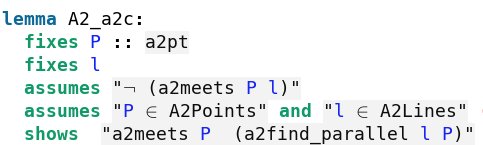
\includegraphics[width=0.5\linewidth]{TEXT/C03/Images/good-statement.png}
\end{figure}

Contrast that with this incorrect lemma statement:
\begin{figure}[h]
    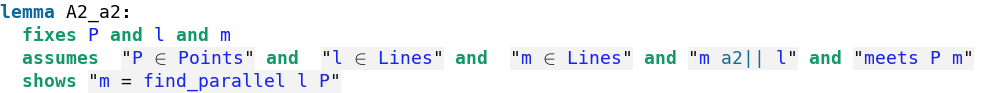
\includegraphics[width=\linewidth]{TEXT/C03/Images/bad-statement.png}
\end{figure}
They really look pretty similar, but in the second lemma, I've used "Points" and "Lines" rather than "A2Points" and "A2Lines". The first two have not been defined, while the second two have. That makes the first two "free" variables -- it's as if my theorem statement said "For all sets Points and Lines, if P is in Points and ..."
That's not what I intended at all. The big clue here is the color: in the first theorem statement, \isi{A2Points} is in black, indicating a bound variable. In the second, \isi{Points} is in blue, indicating a free variable (one that will be implicitly included in a 'forall' at the start of the lemma. (The same goes for \isi{meets} and \isi{find_parallel}.) Informal summary: "Red is horrible. Blue is probably bad." 

\item Check to be sure that you're trying to prove what you're trying to prove. By this I mean "check that the 'shows' part of 'fixes-assumes-shows' actually states the thing you were hoping to prove, rather than something close to it." Copy-paste can make a fool of you here. Free variables, as in the last example, can be a problem. Simple typos can be a problem. One general clue is that if you're trying to prove something that seems easy, but \isi{sledgehammer} can't do it, there's a good chance it's not actually true. Check that all the necessary assumptions are there; check that the desired conclusions express the right thing. Check that the names are all correct. Only after all that should you start to dig deeper. 

\end{itemize}

\chapter{Outline of things still to do, and in what order}
Face up to the fact that it's time to introduce inner and outer syntax and HOL
Read section 2.7 of https://bookdown.org/aleksander_mendoza_drosik/learn-isabelle/fundamentals-of-isabelle.html#query-proofs

How do we use auto and simp? See https://github.com/isabelle-prover/cookbook/blob/master/src/proofs/methods/Chained_Facts.thy

Nested case proofs (e.g., triangle inequality, where we have a <>0, b <>0. Can I "case" on two things? 

What all the colors mean. "Let", pattern matching, and "unknowns". 

and some apply-scripts


Parametrized types; types with constructors; Ballarin/locales for representing mathematical structures. The possibility of contradiction when you make "rules". The challenges of dependent structures.

Teege: bottom of page 45 to top of page 46: difference in what exports from pattern variables or non-pattern variables.



Chapter 3: The tailor. Sets vs types, UNIV, total functions, "undefined"
Writing "backwards" proofs

lemma "2 * (n :: nat) + 1 ≥ n + 1"
proof -
  presume "2 * n ≥ n"
   thus ?thesis
     by simp
next
   show "n ≤ 2 * n"
     by simp
qed
end



Inner vs outer syntax
Why, when I'm proving things, does "try" (or is it try0?) say that there's a counterexample, but it goes away after I add some definitions to the "using".
The "lego" model of 

Chapter 1 edits:
Clean up spivak proofs and lemmas
Tips on "fixes": "fixes n k" is OK. 
Fixes n::nat k ,- not OK
Fixes n::nat and k ← OK
Fixes f::nat => nat <- needs quotes? 
Fixes f:: "nat => nat" <- OK
General: things you're naming can often skip quotes if they're simple, but if you get odd errors, try adding quotes. Example: theorem-names CAN be quoted if you like. Custom says that they almost never are, though. 

What about when you type
lemma "junk":
  fixes f::"nat ⇒ nat"

…you get a warning: Outer syntax error⌂: proposition expected,
but keyword fixes⌂ was found
 The problem isn't that you typed "fixes", it's that you hadn't finished, and need to type "shows" to make a complete theorem-statement. 

THINGS FOR ME TO LEARN

How to improve the Spivak proofs, step by step. 
The just-proved fact is always available, so you can stop with "using n-1"
Sequential arithmetic proofs
Multiple steps in one 'have'


What is available to the various solvers when they do their magic? Auto sometimes fails because I haven't mentioned the definition of lt or ge, etc., but sledgehammer seems to find those things on its own. 

Proving a ton of tiny theorems seems like a Good Thing, but doesn't it make for a combinatorial explosion in the search process?  

Chapter 4: What happens when you define something, or prove a theorem? A whole bunch of new names enter the namespace!

Chapter 3: What various solvers can do well
Chapter 5: Types, sets, and defining functions on sets

Colors (taken from a stackexchange posting by "Mathieu" at https://stackoverflow.com/questions/22635300/what-do-colour-codes-mean-in-isabelle-jedit):

Logic:
blue : free variable
green : bound variable
orange : skolem constant ("free" variables existentially "quantified")
cyan : syntax (not a variable or a constant, like case or if)
Isar Keywords:
sky blue : commands (like lemma, proof or have)
red : tactic-style commands (like apply, done or prefer)
turquoise : statements (like where, fixes, shows or and)
Messages highlighting in output:
red : error
yellow : warning
light blue : info
Highlighting in editor:
red : error
light yellow : current line
gray : quoted text (logic and types)
light gray : comment and formal text (introduced with text or section)
purple : running process on the command (also shown on the right)
pink : unprocessed (outdated) command (also shown on the right)
In general, an underlined command displays a message in the output (possibly associated with an icon and a box on the right). More specifically:
Icons, [boxes] and {in text}:
red exclamation mark [red box] {squiggly red underline} : error
orange exclamation mark [orange box] {squiggly orange underline} : warning
blue i {squiggly blue underline}: information (often provided by automatic tools)
{squiggly gray underline} : the command shows a message in the output
{red text} : comment (like (* This is a comment *))
\chapter*{To Do}
\begin{itemize}
\item 
Stuff isabelle produces: what do def, fun, etc, insert into environment. How do simpset change with each "fun", etc. What does "quotient" and "lifting/transfer" produce? 
\item page 31 of \|https://isabelle.in.tum.de/doc/tutorial.pdf|
\item using sledgehammer: put after "using" or "unfolding" or "have ..." or "show ..." but NOT after "by"
\item in sledgehammer, figure out how to turn on detailed feedback; apparently the magic settings are [verbose, debug] .
\item point people to read the first few pages (up to the "options" section) of the sledgehammer manual: https://isabelle.in.tum.de/dist/doc/sledgehammer.pdf
\item Also: a bunch of nice facts here -- https://stackoverflow.com/questions/21694248/isabelle-why-do-i-get-completely-different-results-when-running-try-versus-sled -- that I might want to incorporate. 
\item explain coding: grey background = isabelle code; purple background = isabelle interface components (buttons, files, panels) or interface-responses (the contents of the 'output' panel, for example), except in the rare cases where these are actual isabelle code; peach background = systems things, like filenames typed into dialog boxes. Because such filenames can also be part of isabelle code, I won't be completely consistent about this, but I'll try to at least be sensible.
\item .Fix spacing in isabelle code style.
\item Move style files to subdirectory
\item Make all latex intermediate files be ignored by git
\item add section on cartouches
\item Fix marginnote to be able to contain "isi" stuff.
\item +For the "sys" and "co" languages, make sure that all characters are un=special (e.g., tildes!)
\item Introduce "Of" and "where" in "using" clauses
\item Why is code "verbatim-like" and can this be fixed? 
\item .Restructure into chapters
\item .define displayed-code macro: Perhaps IC for displayed code? 
\item .Figure out image inclusion
\item .get bibliography working
\item .get non-keyword text in Isabelle source to be ttfamily as well (e.g. presburger)
\item .Define digression-box (add "digression" header)
\item .fix quotes in Isabelle code to be stupid quotes
\item .define clean inline-isabelle macro 
\item .Reduce left margin; increase right margin so marginpars can fit.
\item .get Sys language definition working: fixed wdth font, pale blue background
\end{itemize}

\begin{verbatim}

Pointer to isabelle community cookbook: https://isabelle.systems/cookbook

"value" to use a debugging tool (and warning about things whose values can't be printed)
datatype pointD = Hd | Ad | Bd | Cd| Dd| Ed| Fd| Pd | Qd |Rd
definition PointsD::"pointD set"  where "PointsD = {Hd, Ad, Bd, Cd, Dd, Ed, Fd, Pd, Qd, Rd}"

value "PointsD" produces
"{Hd, Ad, Bd, Cd, Dd, Ed, Fd, Pd, Qd, Rd}"
  :: "pointD set"


"thm" as a debugging tool

Every theorem is a function! Example: 
lemma X: 
  assumes "a > 10"
  assumes "b > 15"
  shows "a + b > 25"
  
shows up as 

[?a > 10] => [?b > 15] => [?a + ?b > 25]

That means you can type X [OF 13 19] and get

[13 > 10] => [19 > 15] => [13 + 19 > 25]

which you can read as "if 13 > 10 adn 19 > 15, then 13 + 19 > 25." Cool!

Using x by y : you can see what's happening here by looking at the state with your cursor just before 'using', just after x, etc. 

tracing simp


How do I write a cases proof for trichotomy? 

\end{verbatim}


\subsection{Doing proofs right}
Once you've done some more Spivak proofs ... we'll move into affine geometry. 
To prove the affine plane on 4 points is an affine plane, we need to show all the axioms hold. The only really messy one is 
\begin{verbatim}
    "¬ affine_plane_data.collinear
           A4Points
           A4Lines
           A4meets Pa Qa Ra"
\end{verbatim}
Proving a negation \textit{could} be done by expanding the definition of collinear (a conjunction of several items), negating it (using blast), and then showing that each of the resulting disjunction elements is false...but one of these is existentially quantified, so it becomes universally quantified, so it requires working through all possible lines one at a time. 

Instead, the right approach is classical contradiction: we assume they ARE collinear, fix a line $n$ that contains all three, and show this leads to nonsense. (A simple way, in this case, is to observe that the cardinality of $n$ must be at least 3, but the cardinatlity of each line in A4 is exactly 2, but we instead work through the details because it's instructive for later proofs, and Isabelle is good at enumerate-and-check approaches.) 

Warning: I want to use ccontr to show the statement above. My first version said
\begin{IS}
proof (rule ccontr)
    assume cHyp: "affine_plane_data.collinear
           A4Points
           A4Lines
           A4meets Pa Qa Ra"
    ...
\end{IS
but that failed badly. Why? Because the thing you assume must be the negation of the thing you want to prove; I should have written
\begin{IS}
proof (rule ccontr)
    assume cHyp: "¬¬affine_plane_data.collinear
    ...
\end{IS
i.e., simply put a negation sign in front of the desired goal. The fact that ¬¬ is the same as "no negations at all" eludes Isabelle (!)

Need to discuss sledgehammer, and how it has access to a million facts, but won't always choose the one you need. Nudging it with a helpful "using" (esp. using XXX [of Y Z W]) can be a big help. Better still (according to Eberl) is to use specific tactics

He says this: "-- I look at proofs in HOL-Algebra and ask myself "why aren't my proofs \newline
-- ever that short?"

Like most things, it's a matter of experience. You just learn how to
write things down in ways that are nice and concise and perhaps easiest
for the automation to deal with. And you learn how to use all the
different tactics for the best effect. I for one am a big fan of doing
every step in Isar by first using a very specific, predictable tactic
like "rule", "intro", "subst" and then getting rid of the arising
subgoals with something more hard-hitting and unfocused like "auto". I
do occasionally use sledgehammer, but perhaps not as much as other
people. I tend to not like the kinds of proofs it creates.

--End of Eberl quote --


tactic to learn: locale_unfolding



Example citation: \cite{latex2e}.

Searching quick tutorial: page 34 of https://isabelle.in.tum.de/doc/tutorial.pdf

\begin{verbatim}
Book design:
Digression: footnote with highlighted background, or margin paragraph
Code: both inline and displayed, in an Isabelle-like format
Topic coloring? Interface, proving, logic, syntax (?)
Chapter summary and high points at end of each chapter


Marginnotes
=====

Homework files: 
ChXX_HWxx_topic.thy
ChXX_HWxx_topic_sol.thy [solutions]

Sample files
ChXX_Sxx_topic.thy
ChXX_Sxx_topic_sol.thy

Code-image-files:
Org by chapter
xxx_topic.png
Xxx.xx_topic.png  (later additions inserted out of sequence)

Scratch files
CHXX_scratchxx

\end{verbatim}


\ignore{ 
Example of a digression:

\digression{Lorem   ipsum. Lorem   ipsum. Lorem   ipsum. Lorem   ipsum. Lorem   ipsum. Lorem   ipsum. Lorem   ipsum. Lorem   ipsum.Lorem   ipsum.Lorem   ipsum.Lorem   ipsum.Lorem   ipsum. }

Example of a digression-with-topic:

\digression[unit measures]{Lorem   ipsum. Lorem   ipsum. Lorem   ipsum. Lorem   ipsum. Lorem   ipsum. Lorem   ipsum. Lorem   ipsum. Lorem   ipsum.Lorem   ipsum.Lorem   ipsum.Lorem   ipsum.Lorem   ipsum. }
And a todo: \todo{remove this}

Example of sys code: \sys{ls ~jfh}.

Example of Inline Isabelle code \isi{theory IbookCh0} and general Isabelle code:
}

"Where do I find a library that does X?" See \verb|https://isabelle.in.tum.de/library/HOL/index.html|

Fix-assume-show notation: you can also include "defines":
\begin{verbatim}
lemma A2_vert5:
  fixes x0 x1 :: real
  defines l_form: ‹l ≡ A2Vertical x0› 
  defines k_form: ‹k ≡ A2Vertical x1›
  assumes ‹a2meets T l› and ‹a2meets T k›
  shows ‹l = k› 
  by (cases T) (use assms in auto)
\end{verbatim}

"How do I create a set using {x | x > 0} notation?" -- see https://isabelle.zulipchat.com/#narrow/channel/238552-Beginner-Questions/topic/Construction.20a.20set

"How should I define my function (with "definition" or "fun" or "abbreviation" perhaps?) and why?" 

"unfolding" vs "using"
Lovely problem for HW2: https://math.stackexchange.com/questions/5031061/prove-that-a-monoid-is-trivial-using-some-specific-conditions/5031092#5031092
\lstset{language=Isabelle}
\begin{lstlisting}
theory IbookCh0
  imports Main EX
begin
end
\end{lstlisting}

\lstset{language=sys}
\begin{lstlisting}
theory IbookCh0
  imports Main EX
begin
end
\end{lstlisting}

\ignore{
lemma "evens": "\<exists> (n::nat) . 2*n > (k::nat)"
  by presburger

lemma "evens2": "\<exists> (n::nat) . 2*n > (k::nat)"
  using evens by auto

lemma "evens3": "\<exists> (n::nat) . 2*n > (k::nat)"
proof -
  have example:"2*(k+1) > k" 
    by simp
  show ?thesis 
    using example by blast
qed
}



\bibliographystyle{abbrv}
\bibliography{ibook}

\end{document}
